%auto-ignore
%\chapter{Appendix}

\chapter[Longitudinal Neuroanatomical Progression of PCA]{Longitudinal Neuroanatomical Progression of Posterior Cortical Atrophy}
\label{sec:adni_extra_appendix}

% \tikzset{every picture/.append style={scale=0.6}}

% scale parameter for the font size in the circles
\newcommand*{\scaleLabelImg}{0.7}
\begin{figure}
  \centering
  \includegraphics*[scale=\scaleLabelImg]{images/Mid-Lateral_surface3.eps}
  \caption[Labels of the different areas analysed in the EBM progression snapshots]{Labels of the different areas analysed in the EBM progression snapshots from chapter \ref{chapter:pca}. }
  \label{fig:ebmSnapLabels}
\end{figure}


Description of the labels shown in figure \ref{fig:ebmSnapLabels}:
\begin{itemize}
\item Frontal Lobe (FL)
        \begin{itemize}
        \item Lateral Surface
            \begin{itemize}
            \item Frontal Pole (FRP)
            \item Superior Frontal Gyrus (SFG)
            \item Middle Frontal Gyrus (MFG)
            \item Opercular part of the Inferior Frontal Gyrus (OpIFG)
            \item Orbital part of the Inferior Frontal Gyrus (OrIFG)
            \item Triangular part of the Inferior Frontal Gyrus (TrIFG)
            \item Precentral Gyrus (PrG)    
            \end{itemize}
        \item Medial Surface
            \begin{itemize}
            \item Superior Frontal Gyrus, medial segment (MSFG)
            \item Supplementary Motor Cortex (SMC)
            \item Medial Frontal Cortex (MFC)
            \item Gyrus Rectus (GRe) 
            \item Subcallosal Area (SCA)
            \item Precentral Gyrus (MPrG)
            \end{itemize}
        \item Inferior Surface
            \begin{itemize}
            \item Anterior Orbital Gyrus (AOrG)
            \item Medial Orbital Gyrus (MOrG)
            \item Lateral Orbital Gyrus (LOrG)
            \item Posterior Orbital Gyrus (POrG)
            \end{itemize}
        \item Opercular Region 
            \begin{itemize}
            \item Frontal Operculum (FO)
            \item Central Operculum (CO)
            \item Parietal Operculum (PO)
            \end{itemize}
        \item Insular Region
            \begin{itemize}
            \item Anterior Insula (AIns)
            \item Posterior Insula (PIns)
            \end{itemize}
        \end{itemize}
        
    \item Temporal Lobe (TL)
        \begin{itemize}
        \item Lateral Surface
            \begin{itemize}
            \item Temporal Pole (TMP)
            \item Superior Temporal Gyrus (STG)
            \item Middle Temporal Gyrus (MTG)
            \item Inferior Temporal Gyrus (ITG)
            \end{itemize}
        \item Supratemporal Surface
            \begin{itemize}
            \item Planum Polare (PP)
            \item Transverse Temporal Gyrus (TTG)
            \item Planum Temporal (PT)
             \end{itemize}
        \item Inferior Surface
            \begin{itemize}
            \item Fusiform Gyrus (FuG)
            \end{itemize}
        \end{itemize}
    \item Parietal lobe (PL)
        \begin{itemize}
        \item Lateral Surface
            \begin{itemize}
            \item Postcentral Gyrus (PoG)
            \item Supramarginal Gyrus (SMG)
            \item Superior Parietal Lobule (SPL)
            \item Angular Gyrus (AnG)
            \end{itemize}
        \item Medial Surface
            \begin{itemize}
            \item Postcentral Gyrus, medial segment (MPoG)
            \item Precuneus (PCu)
            \end{itemize}
        \end{itemize}
    
    \item Occipital Lobe (OL)
        \begin{itemize}
        \item Lateral Surface
            \begin{itemize}
            \item Superior Occipital Gyrus (SOG)
            \item Inferior Occipital Gyrus (IOG)
            \item Middle Occipital Gyrus (MOG)
            \item Occipital Pole (OCP)
            \end{itemize}
        \item Inferior Surface
            \begin{itemize}
            \item Occipital Fusiform Gyrus (OFuG)
            \end{itemize}
        \item Medial Surface
            \begin{itemize}
            \item Cuneus (Cun)
            \item Calcarine Cortex (Calc)
            \item Lingual Gyrus (LiG)
            \end{itemize}
        \end{itemize}
    
    \item Limbic Cortex (LC)
        \begin{itemize}
        \item Cingulate Cortex
            \begin{itemize}
            \item  Anterior cingulate gyrus (ACgG)
            \item Middle cingulate gyrus (MCgG)
            \item Posterior cingulate gyrus (PCgG)
            \end{itemize}
        \item Medial Temporal Cortex
            \begin{itemize}
            \item Parahippocampal Gyrus (PHG)
            \item Entorhinal Area (Ent)
            \end{itemize}
        \end{itemize}
    
\end{itemize}


\begin{figure}
\centering
  \begin{subfigure}{\textwidth}
  \centering
 \textbf{\large{\mbox{Posterior Cortical Atrophy}}}
 
 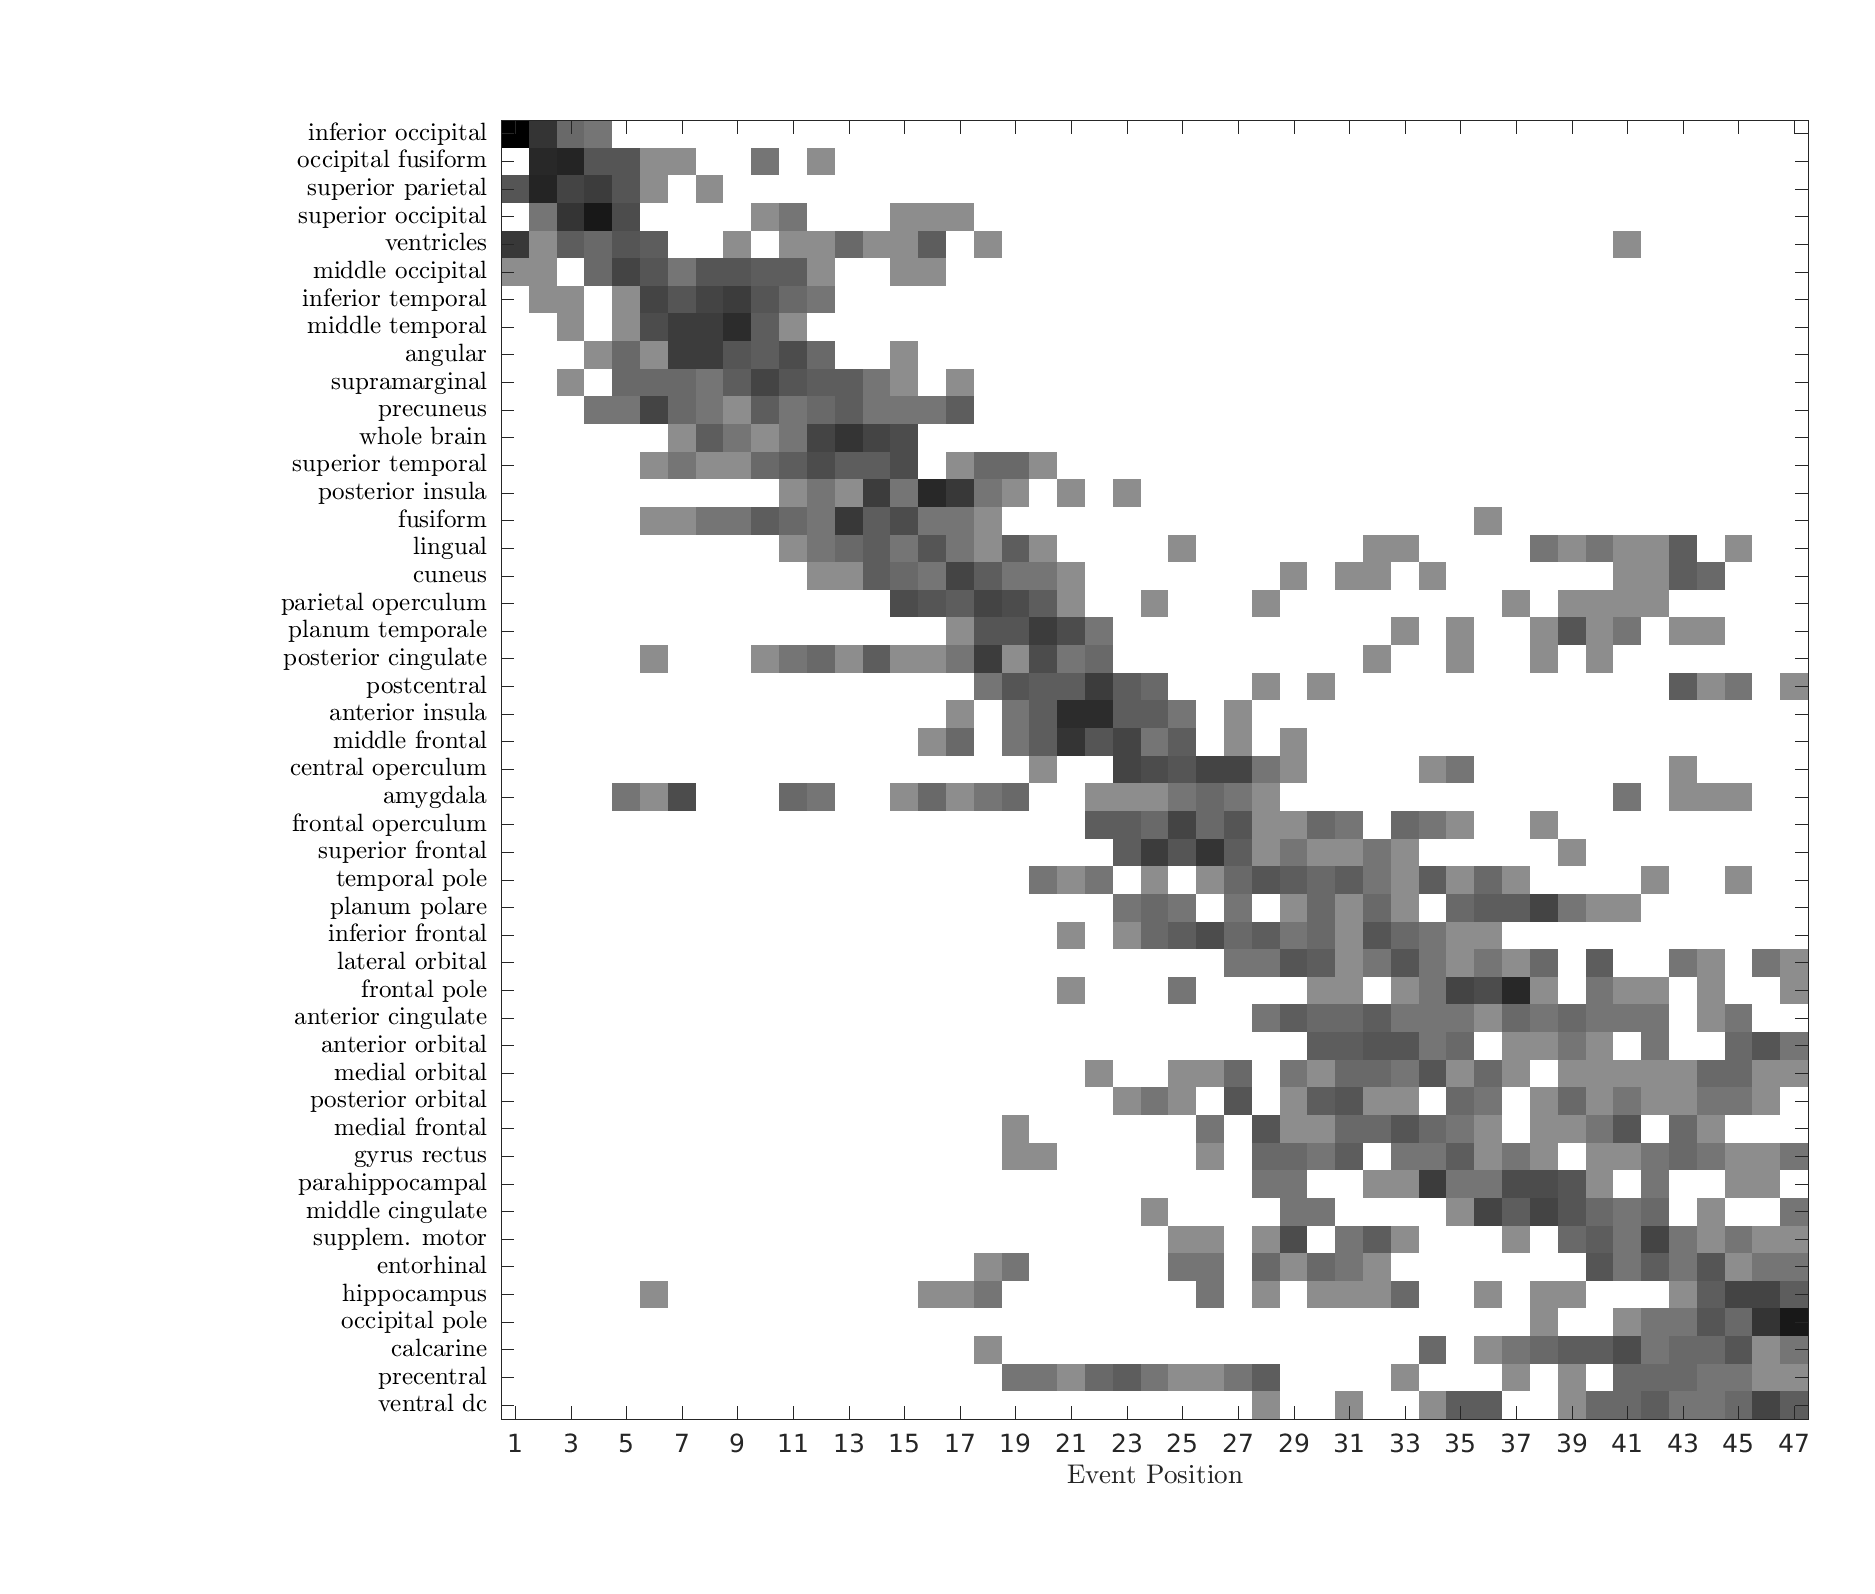
\includegraphics[width=0.7\textwidth,trim=100 30 0 50,clip]{\pcaPaperFigs/bootPosVarAllPCA.png}
 \end{subfigure}
 \vspace{1em}
 
 \begin{subfigure}{\textwidth}
  \centering
  \textbf{\large{\mbox{Typical Alzheimer's Disease}}}
  
 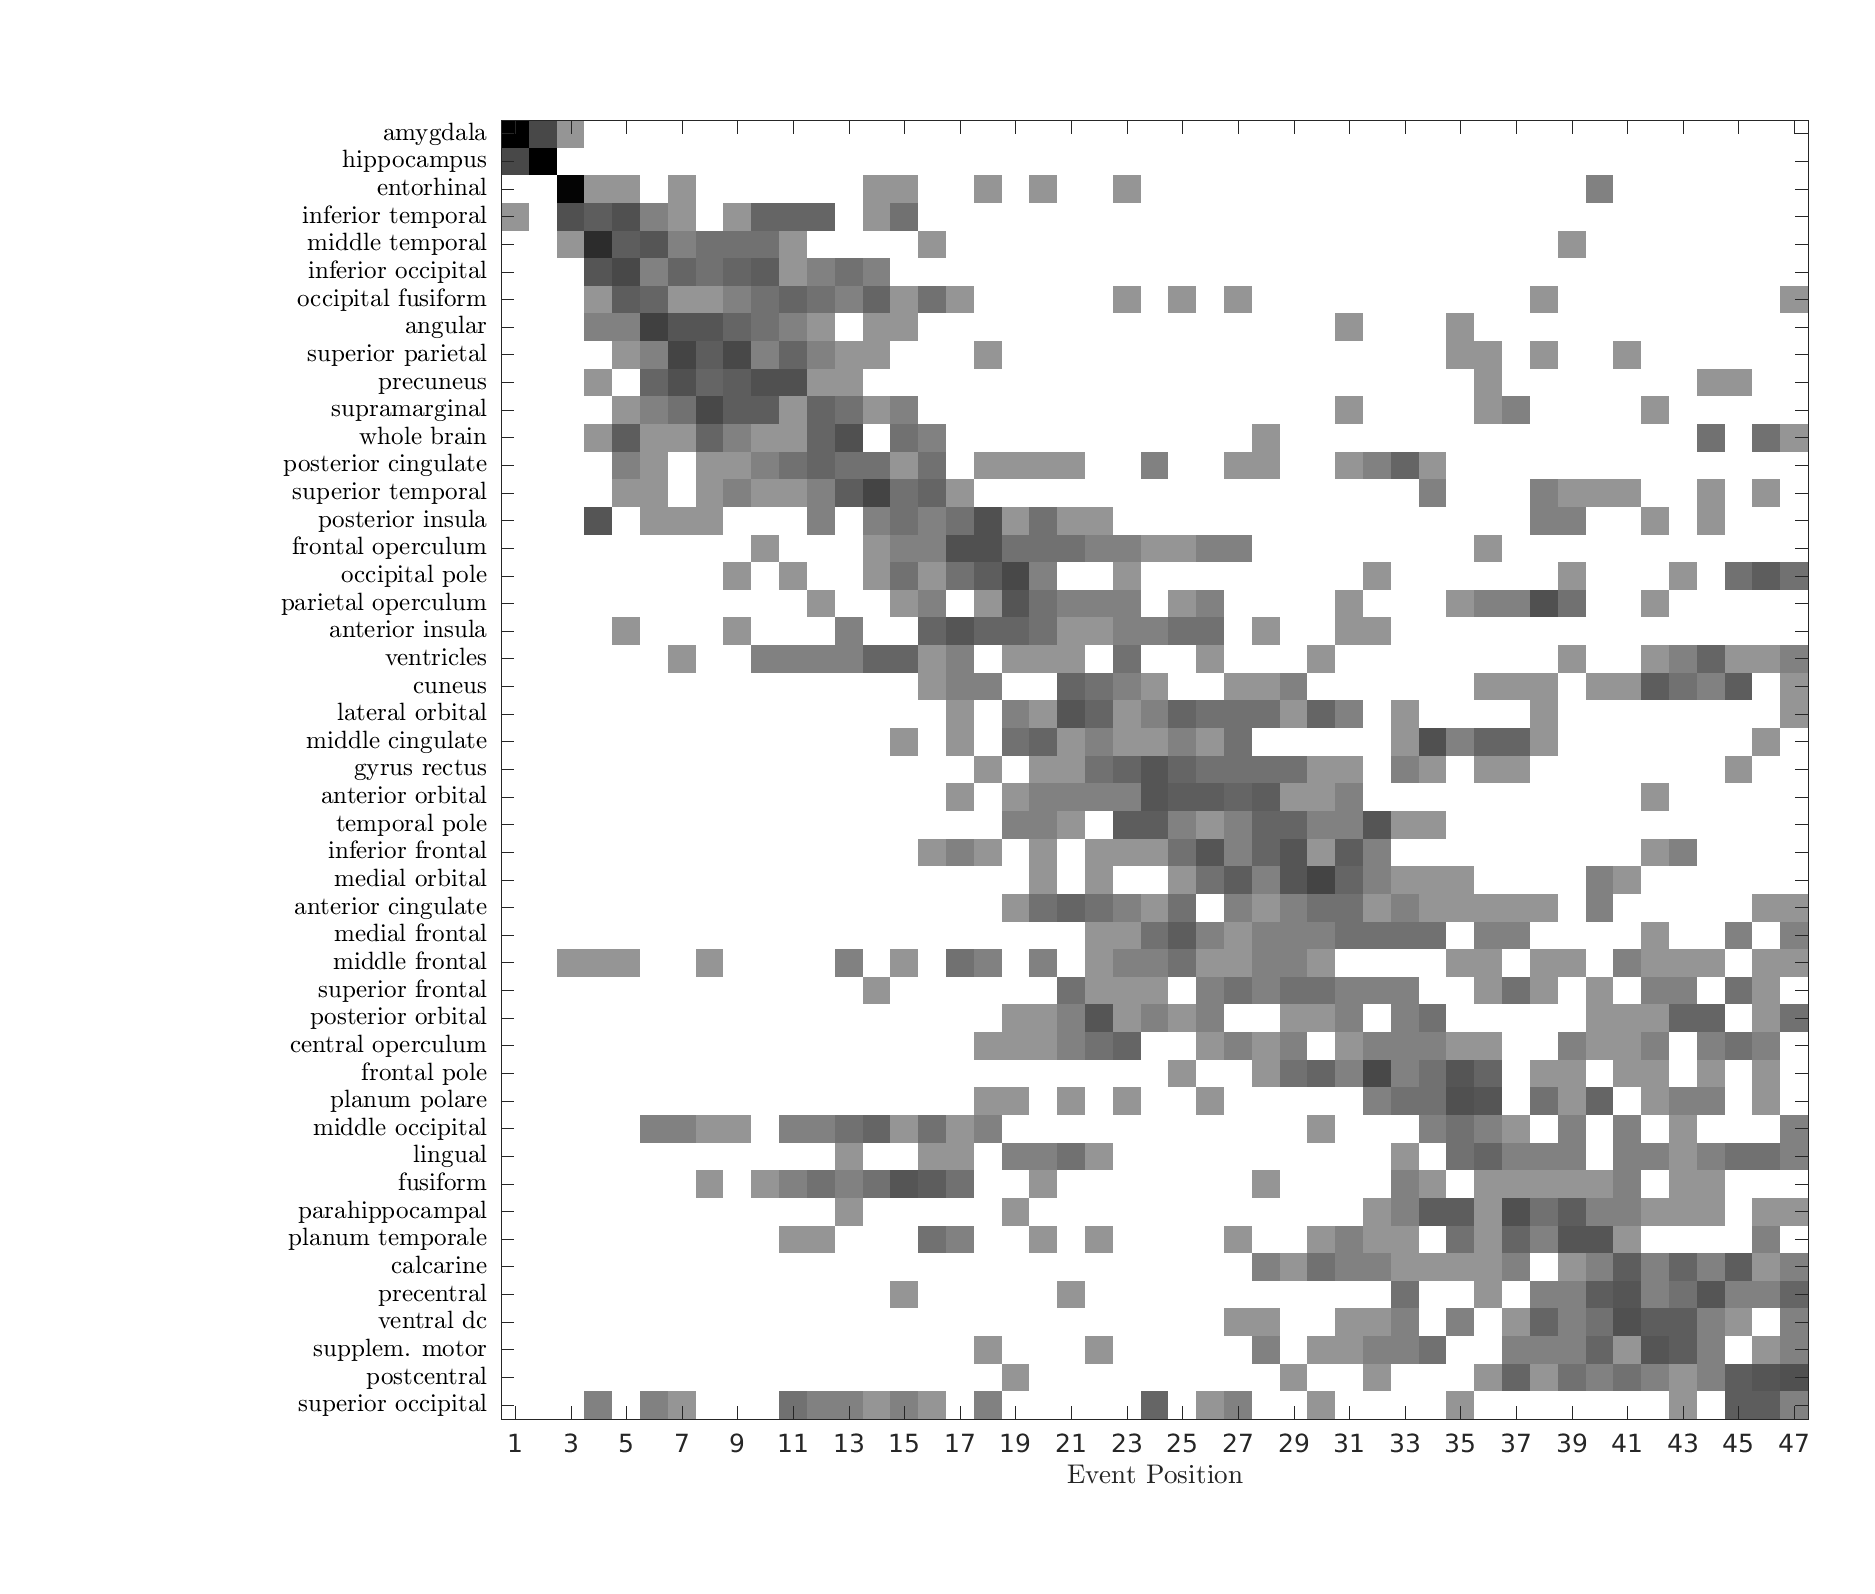
\includegraphics[width=0.7\textwidth,trim=100 30 0 50,clip]{\pcaPaperFigs/bootPosVarAllAD.png}
 \end{subfigure}
 \caption[EBM bootstrap samples of the atrophy sequence for PCA and tAD]{Bootstrap samples of the atrophy sequence as estimated by the event-based model, for the PCA and typical AD cohorts. The maximum likelihood sequences were estimated using the EBM from 100 bootstrap datasets, with replacement, stratified by diagnosis.}
 \label{fig:bootPosVarAllPcaAd}
\end{figure}

\begin{figure}
\centering
  \begin{subfigure}{\textwidth}
  \centering
 \textbf{\large{\mbox{Posterior Cortical Atrophy}}}
 
 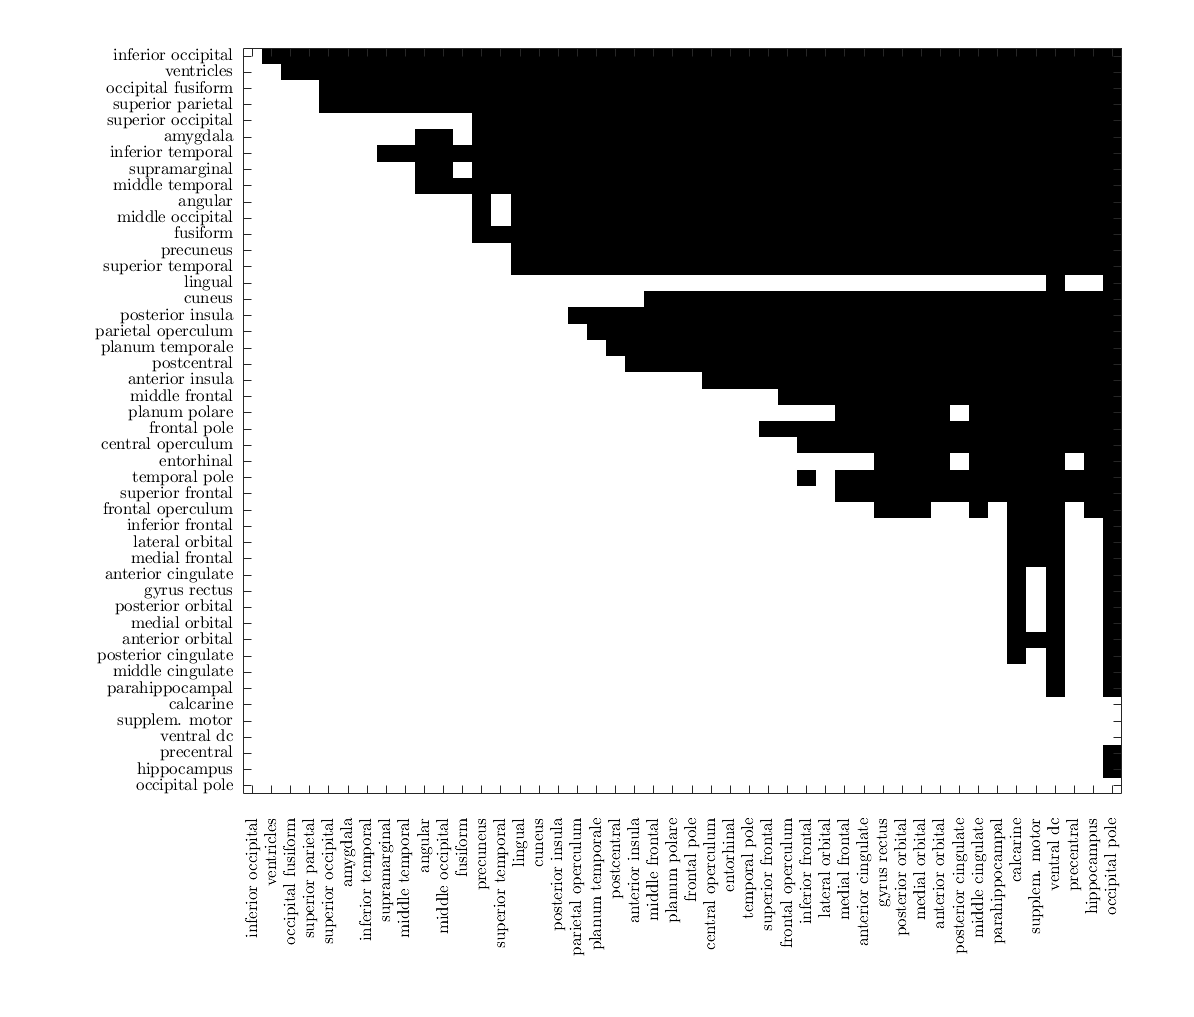
\includegraphics[width=0.7\textwidth,trim=50 30 0 30,clip]{\pcaPaperFigs/statTestPCA.png}
 \end{subfigure}
 \vspace{1em}
 
 \begin{subfigure}{\textwidth}
  \centering
  \textbf{\large{\mbox{Typical Alzheimer's Disease}}}
  
 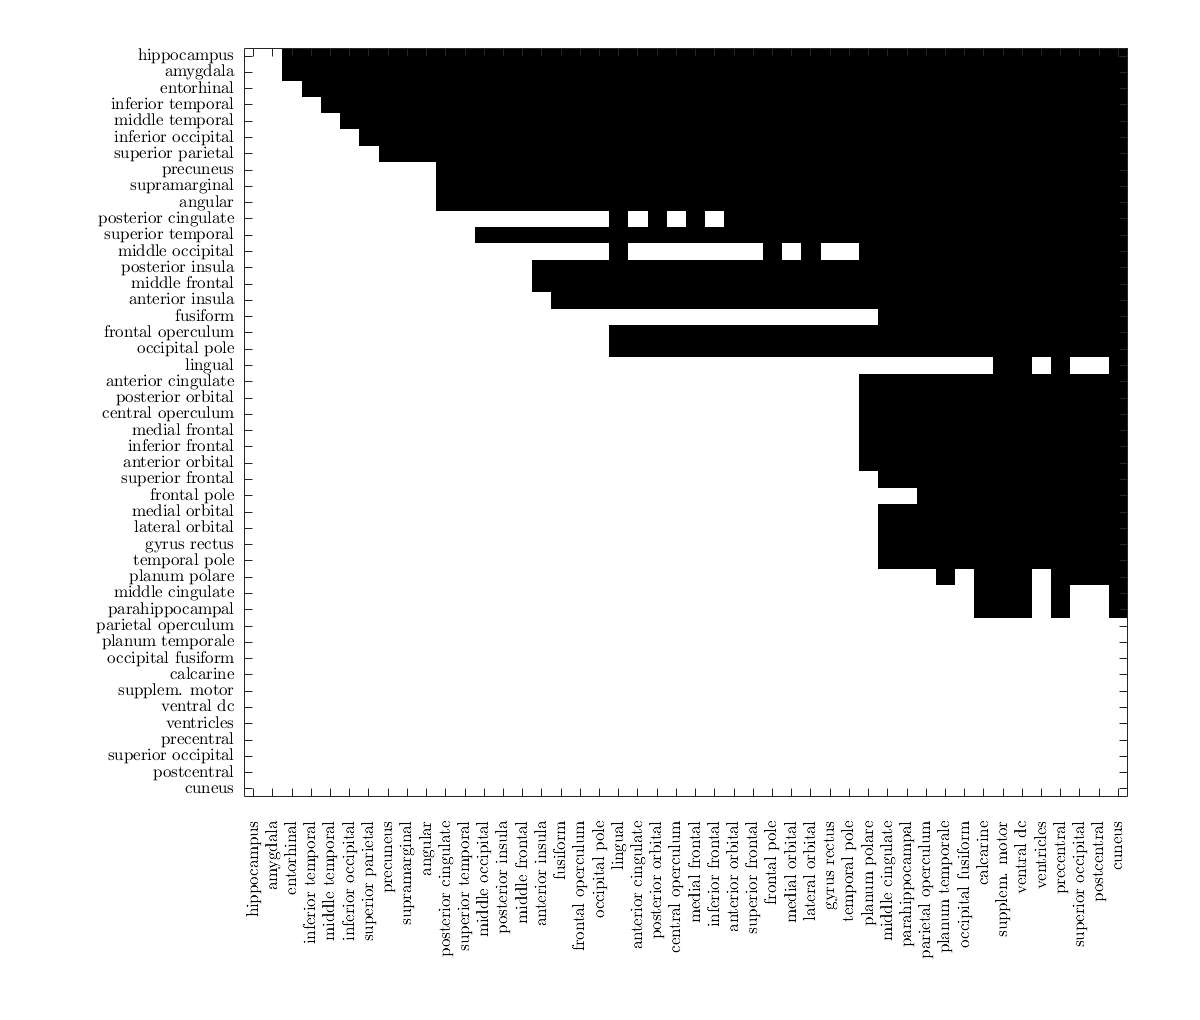
\includegraphics[width=0.7\textwidth,trim=50 30 0 30,clip]{\pcaPaperFigs/statTestAD.png}
%  \caption{}
 \end{subfigure}
 \caption[Hypothesis testing of ordering of events within PCA and tAD]{Hypothesis testing of ordering of events within PCA (top) and typical AD (bottom). We sampled 10,000 sequences from the EBM posterior using MCMC sampling and only kept every 1/100 in order to remove correlation between samples.  We applied the non-parametric paired Wilcoxon signed rank test for every pair of biomarkers (x,y). The null hypothesis is defined as H0: event A (Y-axis) becomes abnormal at the same time as event B (X-axis), while the alternative hypothesis H1: event A (Y-axis) become abnormal before event B (X-axis). The black squares show the pair of biomarkers where the null hypothesis was rejected at alpha=0.05/(N*(N-1)/2), thus surviving Bonferroni correction.}
  \label{fig:statTestPcaAd}
\end{figure}



\begin{figure}
\centering
  \begin{subfigure}[t]{0.48\textwidth}
  \centering
 \textbf{\large{\mbox{Basic visual impairment group}}}
    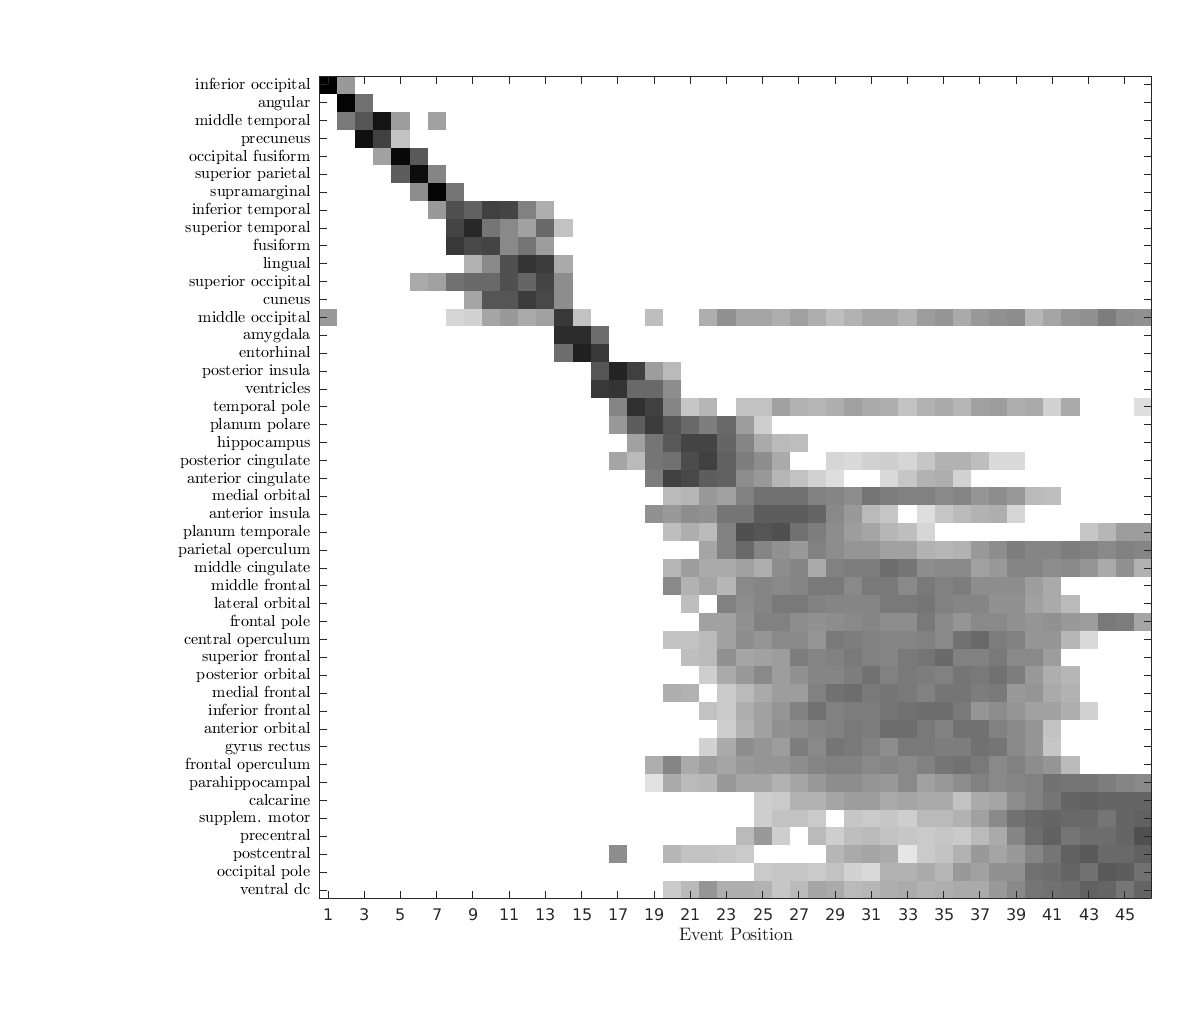
\includegraphics[width=1.2\textwidth,trim=50 30 0 50,clip]{\pcaPaperFigs/posVarianceMatrixEAR.png}
 \end{subfigure}
 
  \begin{subfigure}[t]{0.48\textwidth}
  \centering
 \textbf{\large{\mbox{Space perception impairment group}}}
 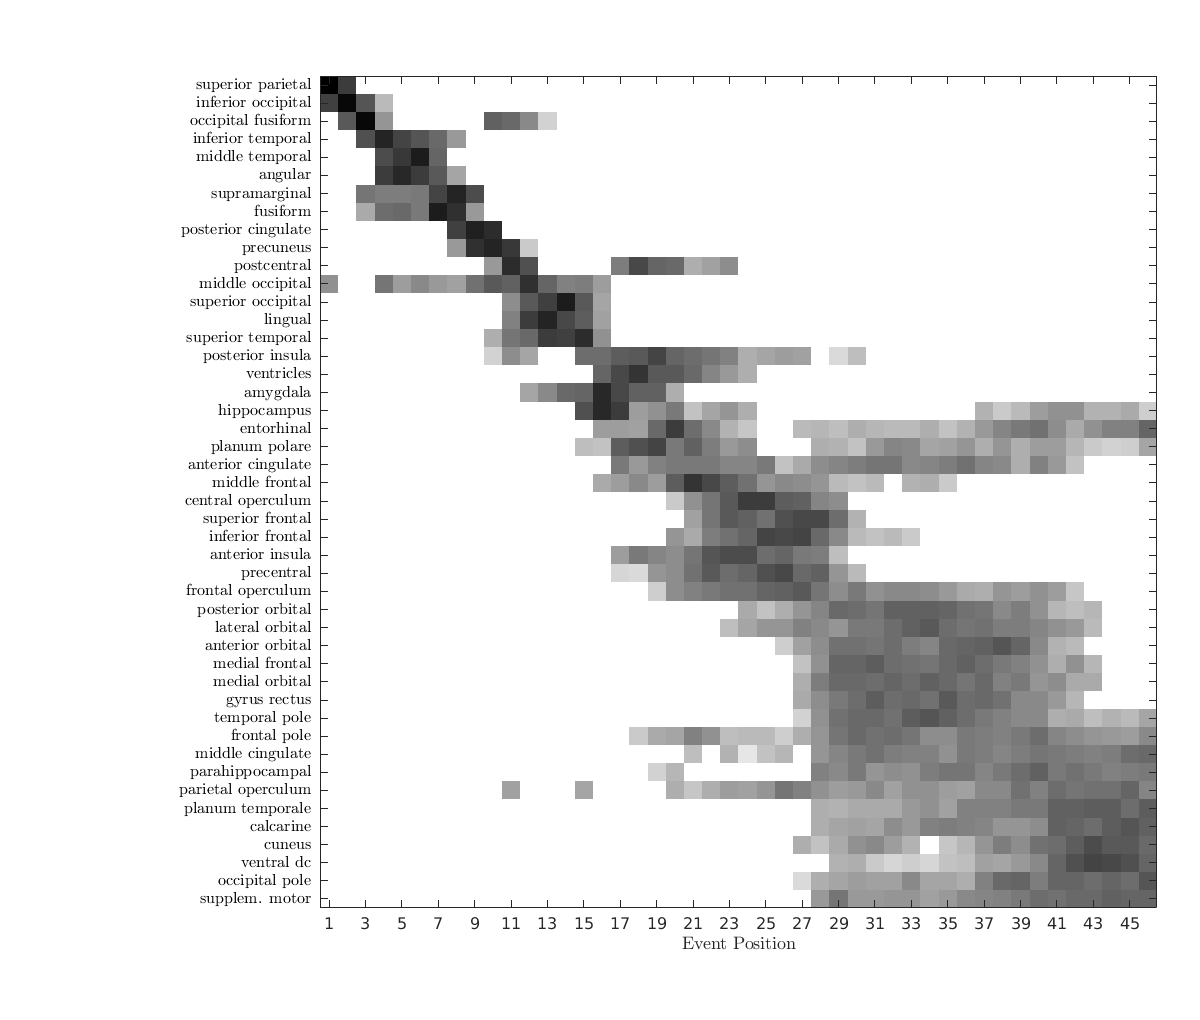
\includegraphics[width=1.2\textwidth,trim=50 30 0 50,clip]{\pcaPaperFigs/posVarianceMatrixSPA.png}
 \end{subfigure}

\begin{subfigure}[t]{0.48\textwidth}
\centering
   \textbf{\large{\mbox{Object perception impairment group}}}
 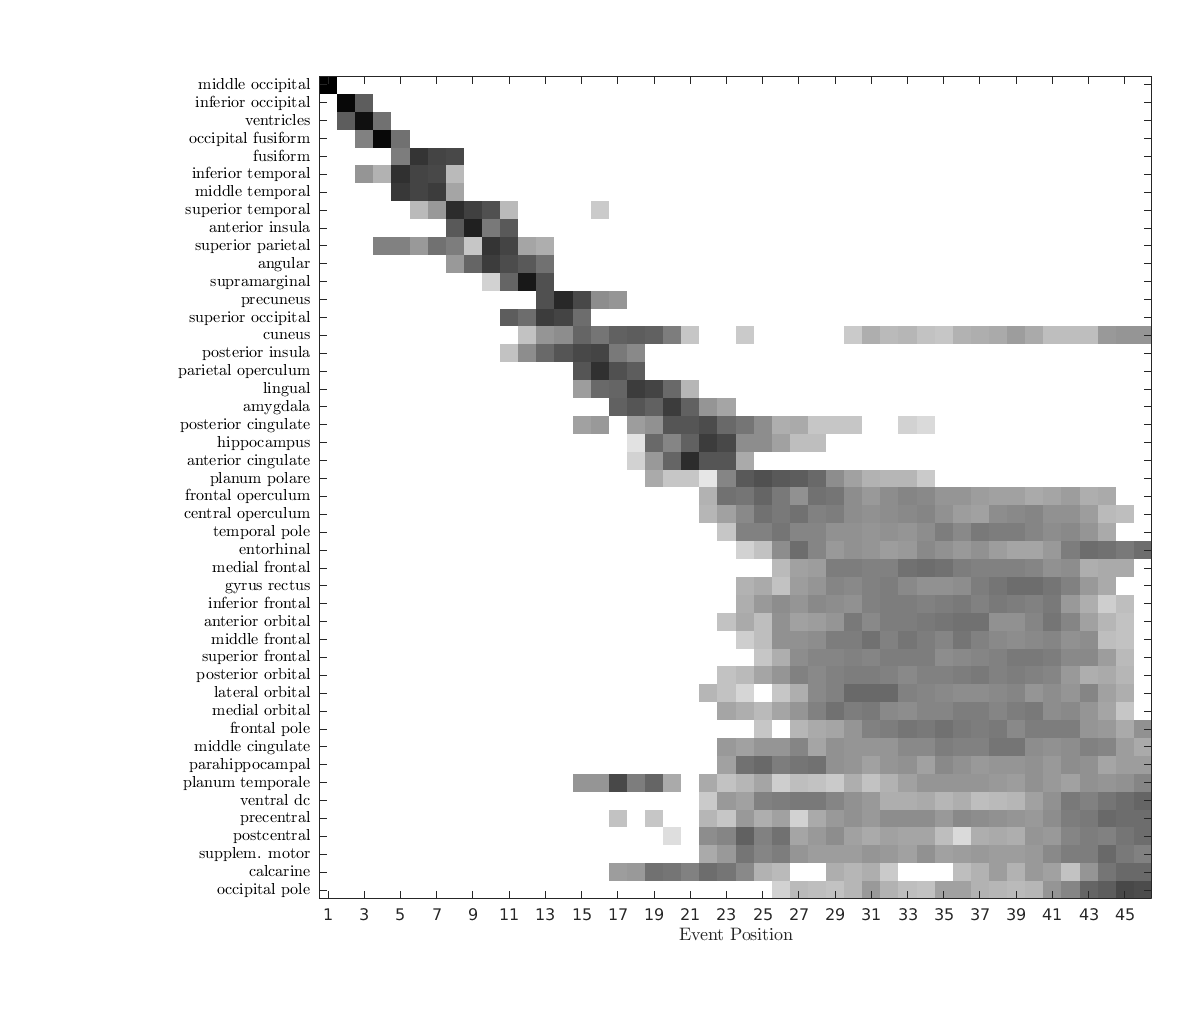
\includegraphics[width=1.2\textwidth,trim=50 30 0 50,clip,valign=t]{\pcaPaperFigs/posVarianceMatrixPER.png}
 \end{subfigure}
 \caption[Positional variance diagram estimated by the event-based model, for three PCA sugroups]{Positional variance diagram estimated by the event-based model, for the three PCA sugroups: Basic visual impairment group, Space perception impairment and Object perception impairment.}
   \label{fig:posVarianceMatrixEarSpaPer}
\end{figure}



\begin{figure}
\centering
  \begin{subfigure}[t]{0.48\textwidth}
  \centering
 \textbf{\large{\mbox{Basic visual impairment group}}}
    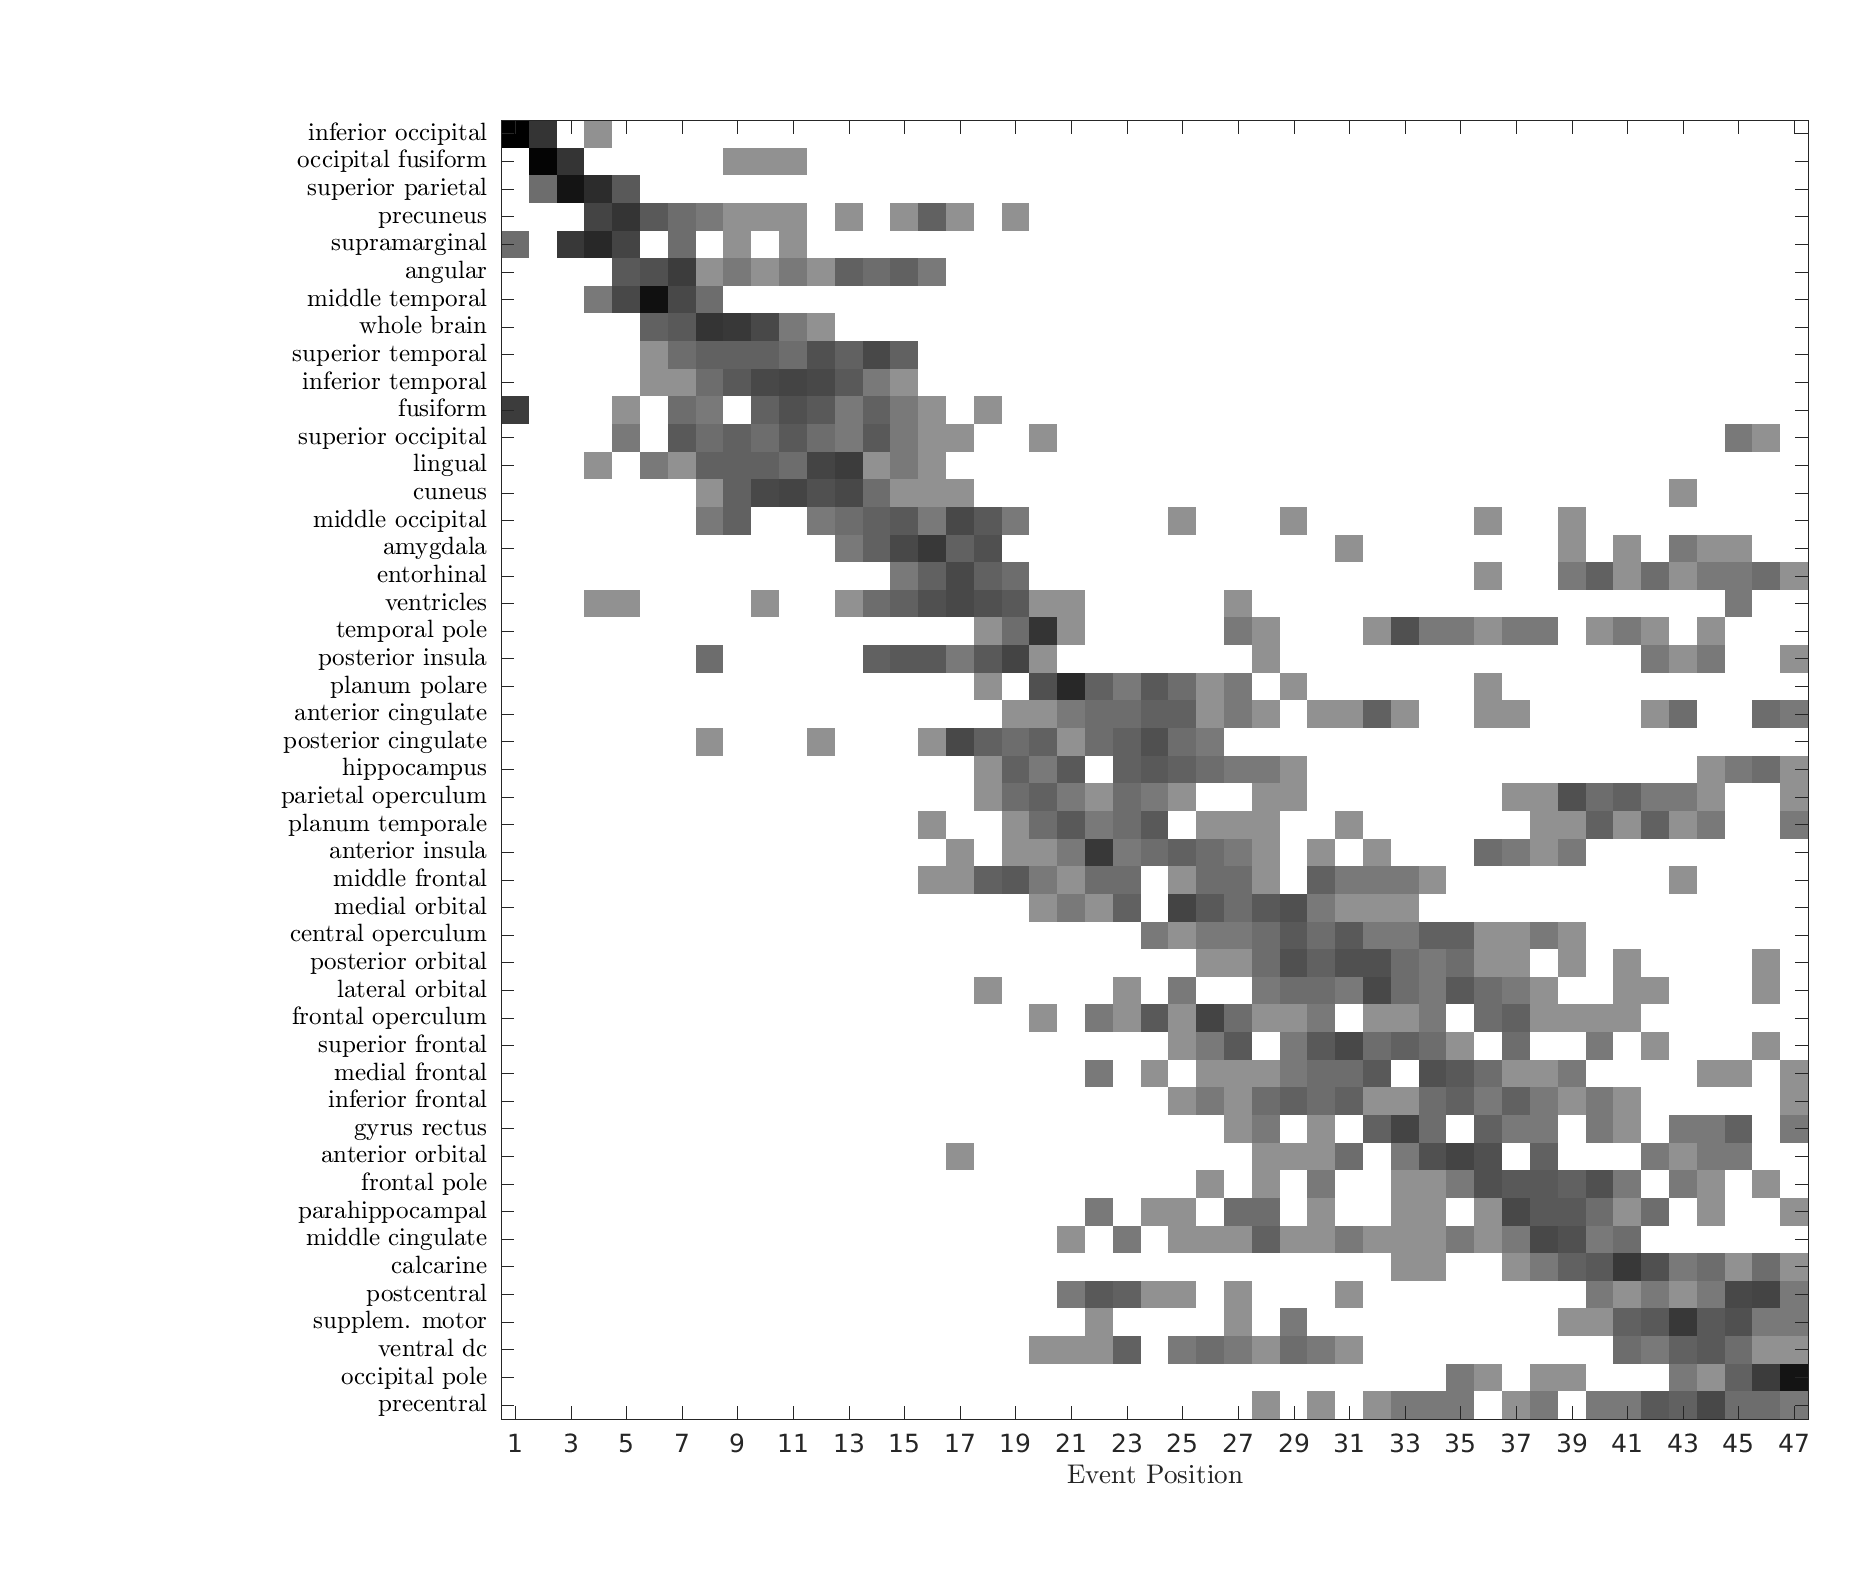
\includegraphics[width=1.2\textwidth,trim=50 30 0 50,clip]{\pcaPaperFigs/bootPosVarAllEAR.png}
 \end{subfigure}
 
  \begin{subfigure}[t]{0.48\textwidth}
  \centering
 \textbf{\large{\mbox{Space perception impairment group}}}
 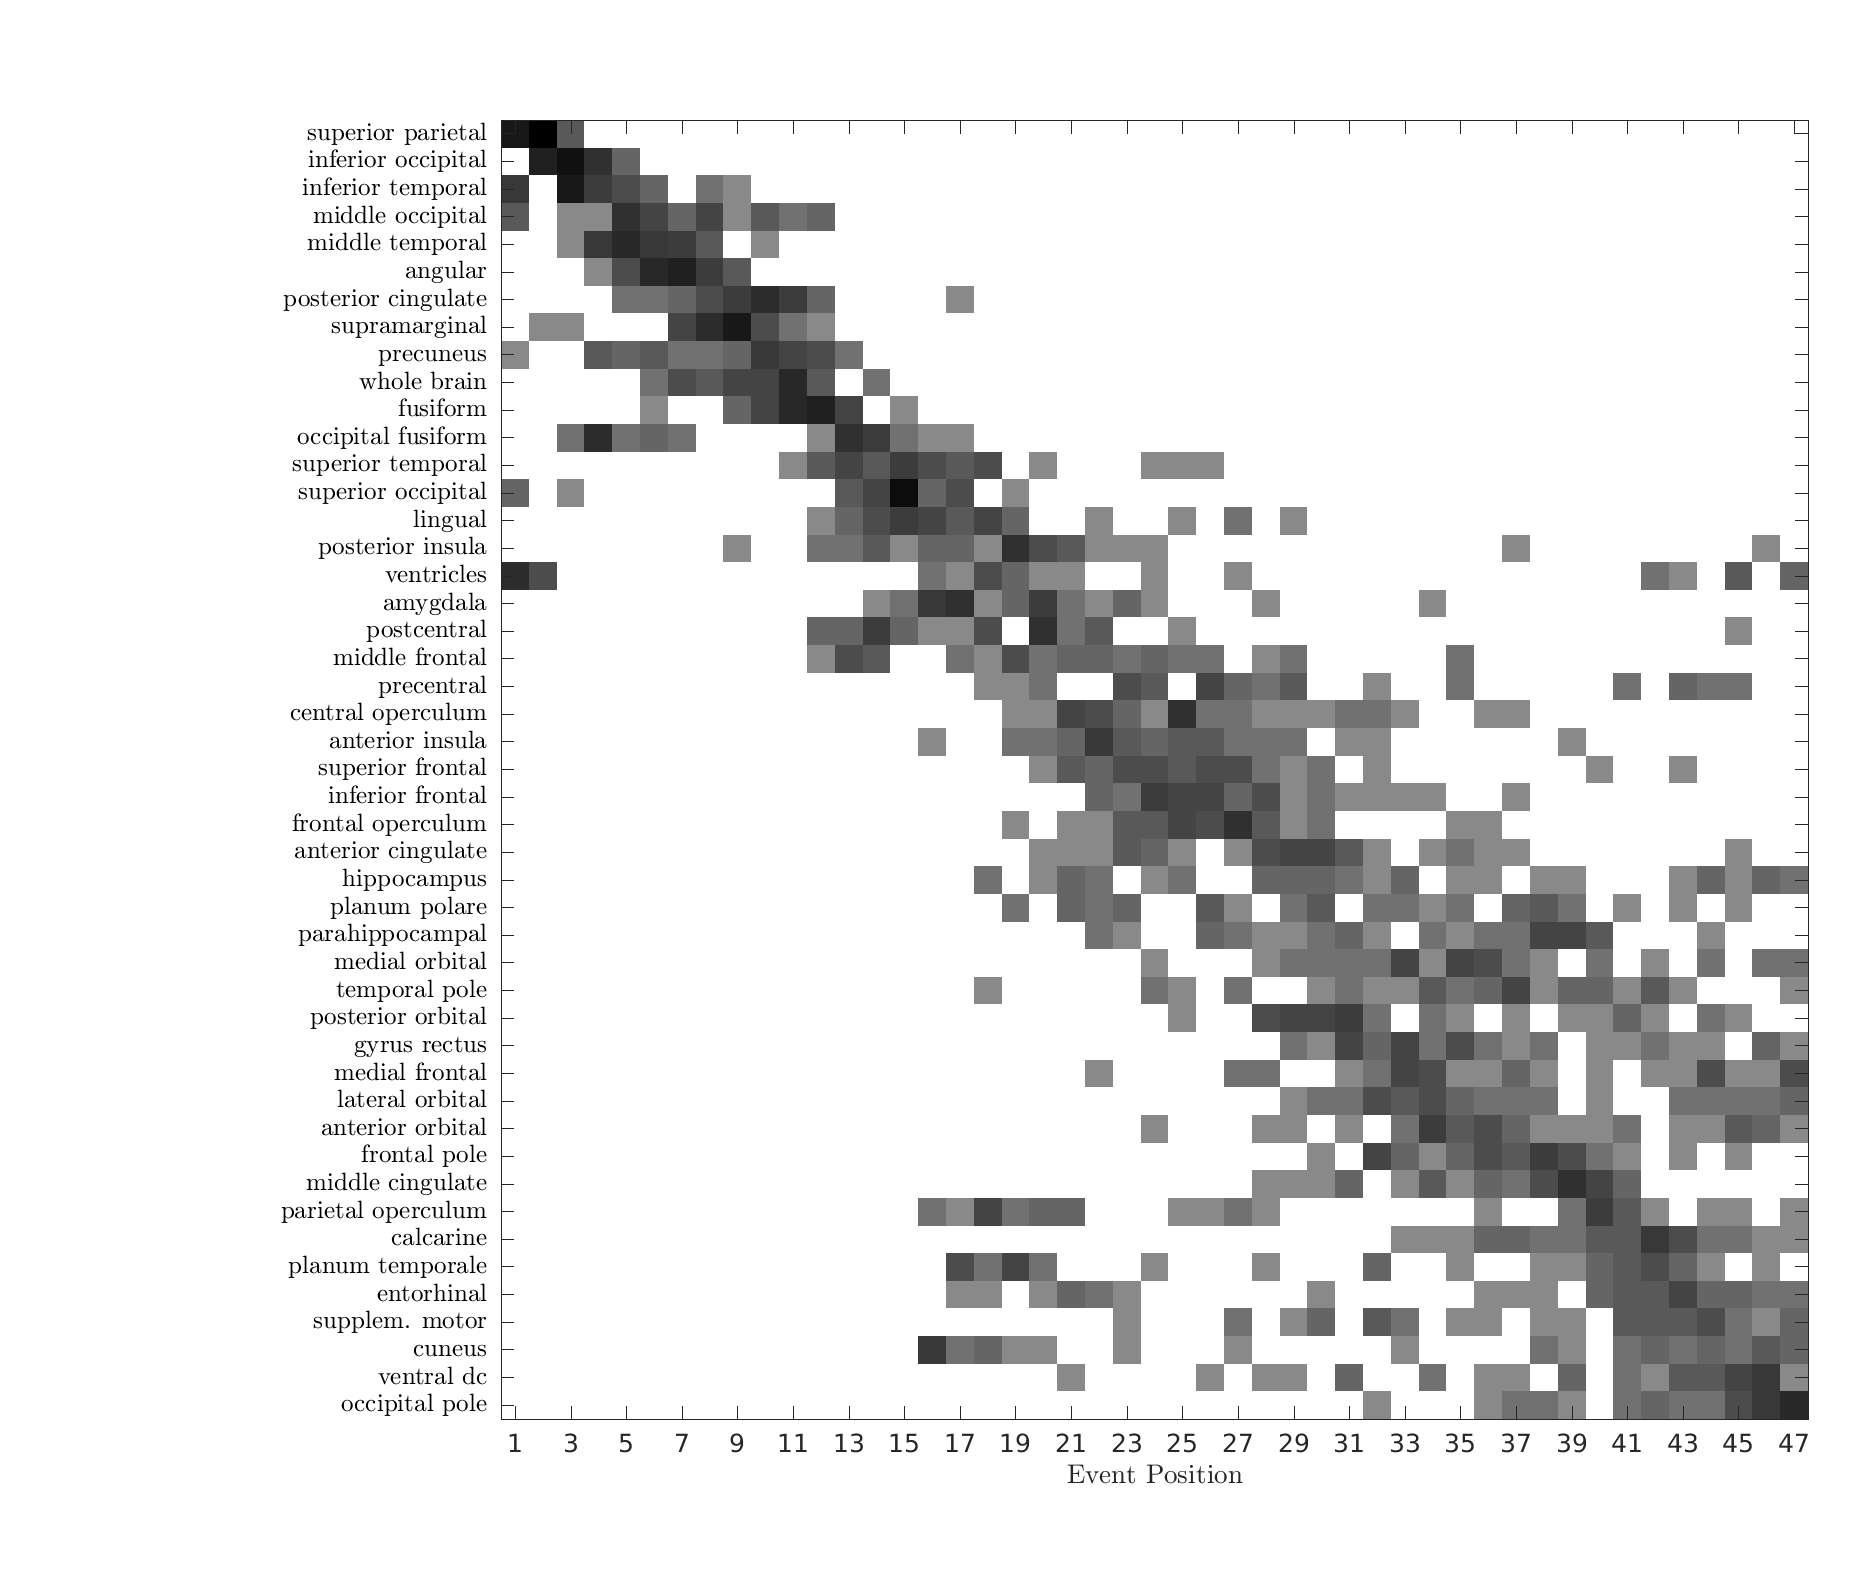
\includegraphics[width=1.2\textwidth,trim=50 30 0 50,clip]{\pcaPaperFigs/bootPosVarAllSPA.png}
 \end{subfigure}

\begin{subfigure}[t]{0.48\textwidth}
\centering
   \textbf{\large{\mbox{Object perception impairment group}}}
 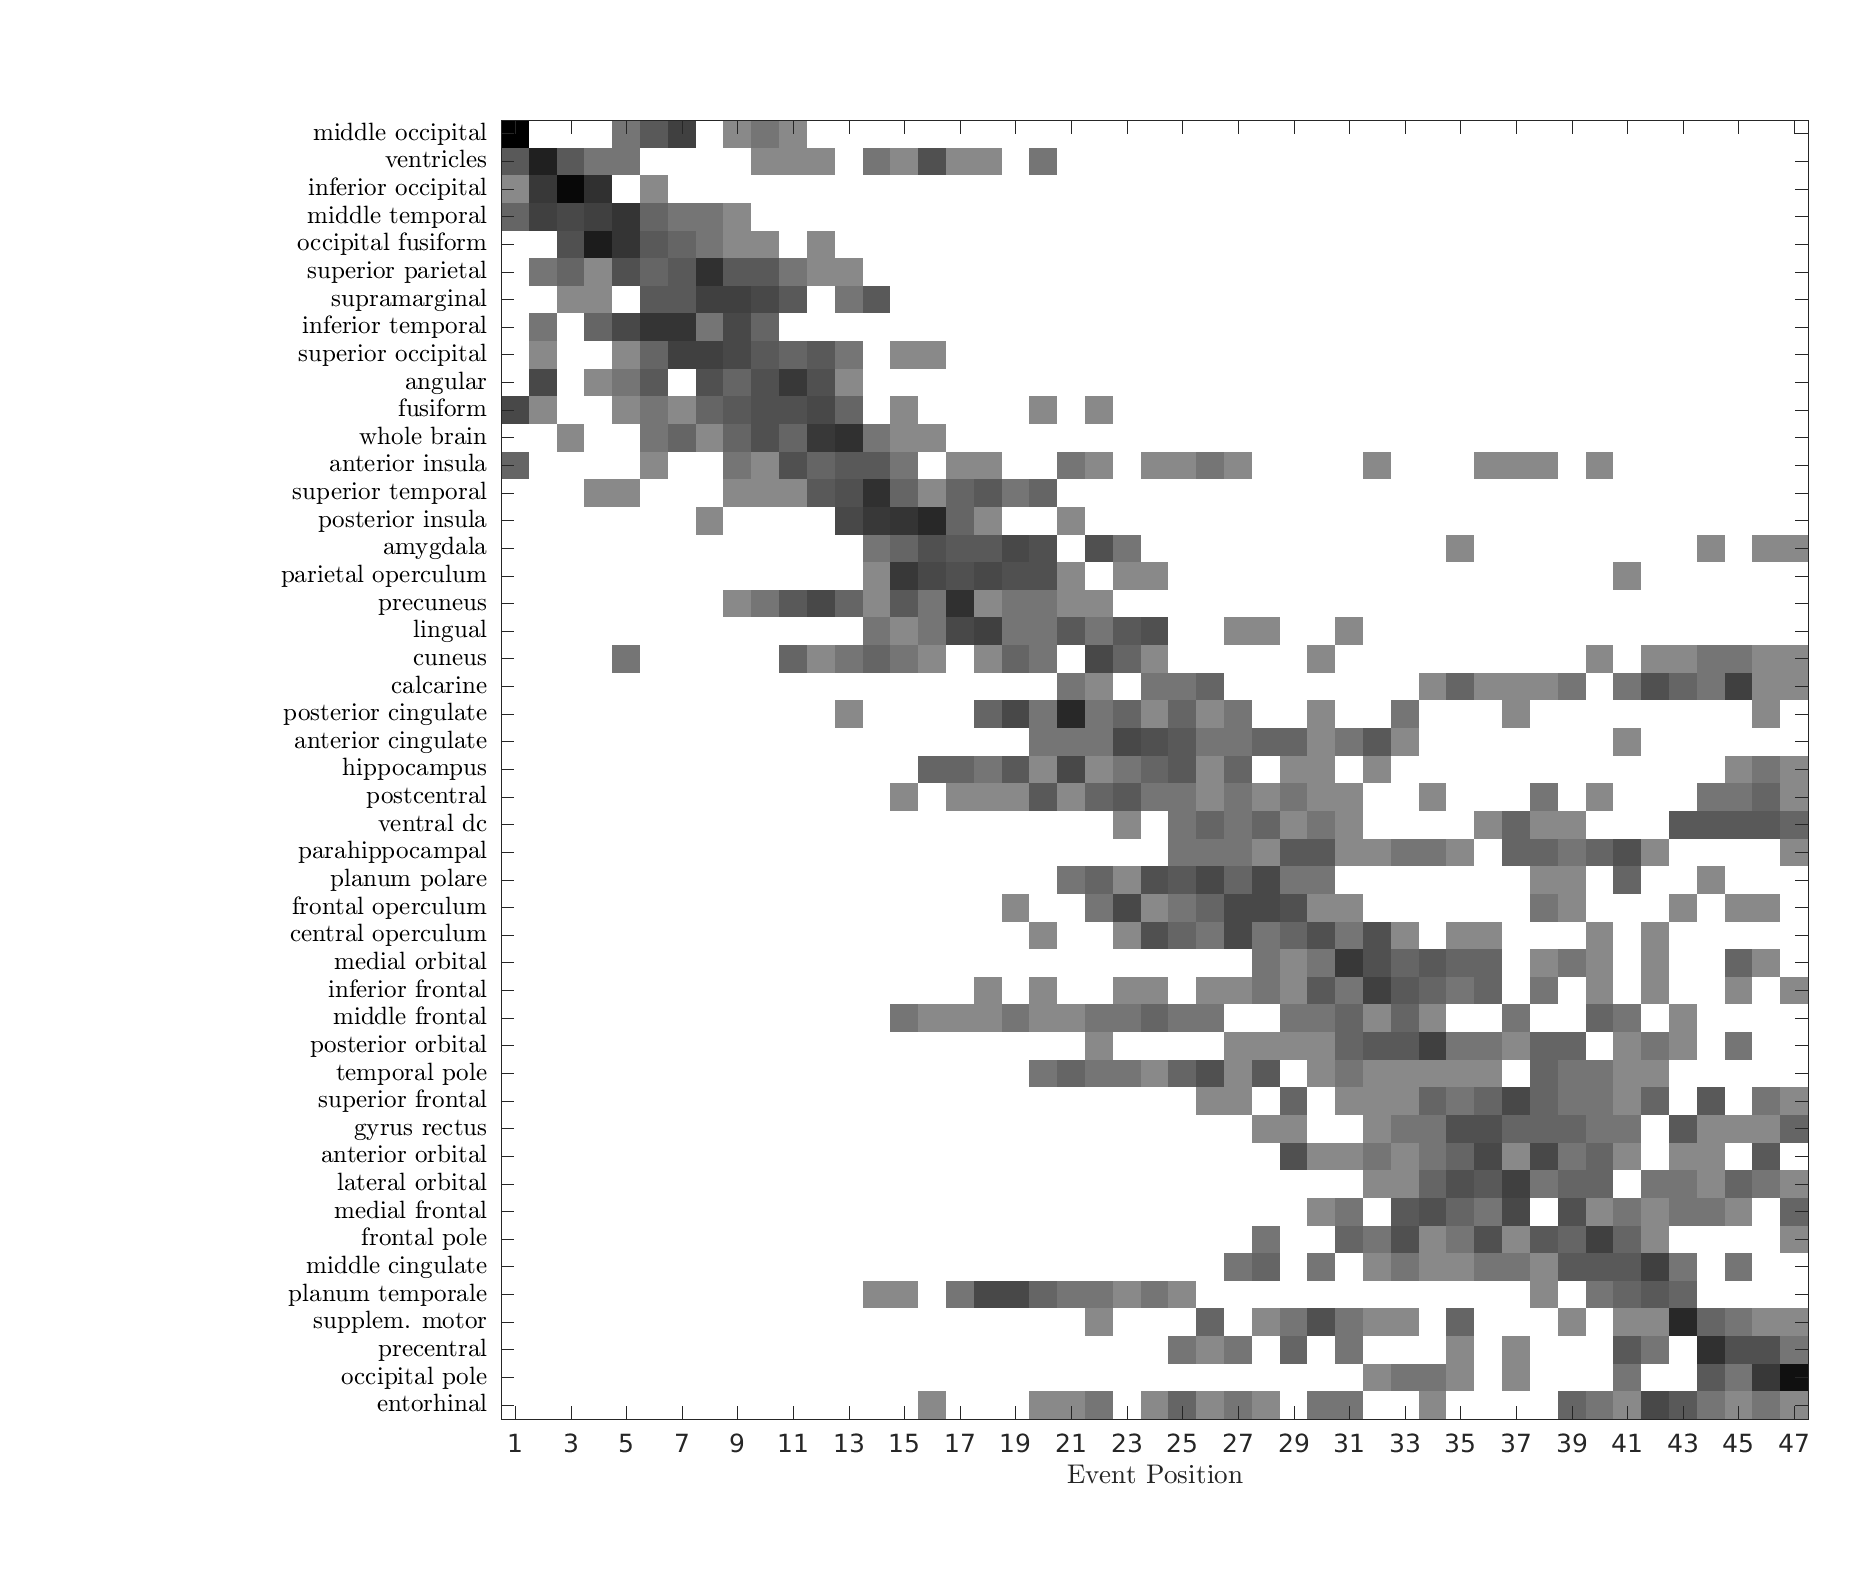
\includegraphics[width=1.2\textwidth,trim=50 30 0 50,clip,valign=t]{\pcaPaperFigs/bootPosVarAllPER.png}
 \end{subfigure}
 \caption[EBM bootstrap samples of the atrophy sequence, for three PCA subgroups]{Bootstrap samples of the atrophy sequence as estimated by the event-based model, for the three PCA sugroups: Basic visual impairment group, Space perception impairment and Object perception impairment.}
 \label{fig:bootPosVarAllEarSpaPer}
\end{figure}


\begin{figure}
\centering
  \begin{subfigure}[t]{0.48\textwidth}
  \centering
 \textbf{\large{\mbox{Basic visual impairment group}}}
    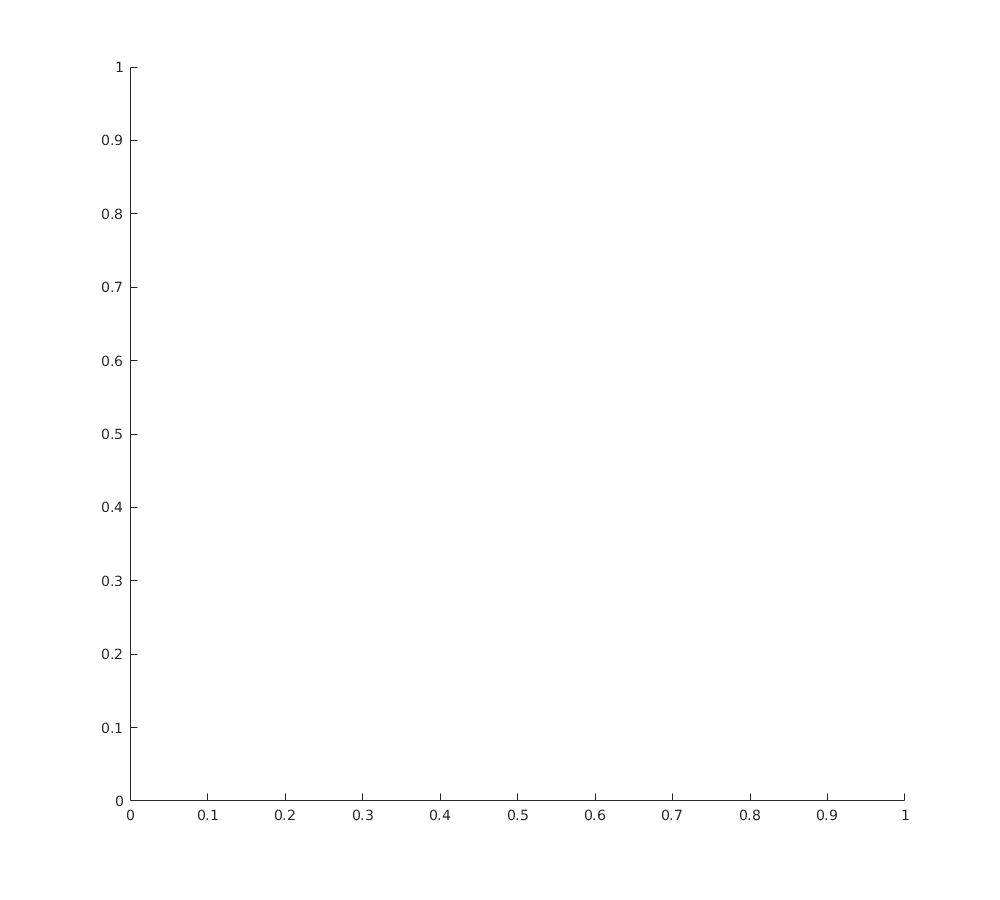
\includegraphics[width=1.2\textwidth,trim=50 30 0 30,clip]{\pcaPaperFigs/statTestEAR.png}
 \end{subfigure}
 
  \begin{subfigure}[t]{0.48\textwidth}
  \centering
 \textbf{\large{\mbox{Space perception impairment group}}}
 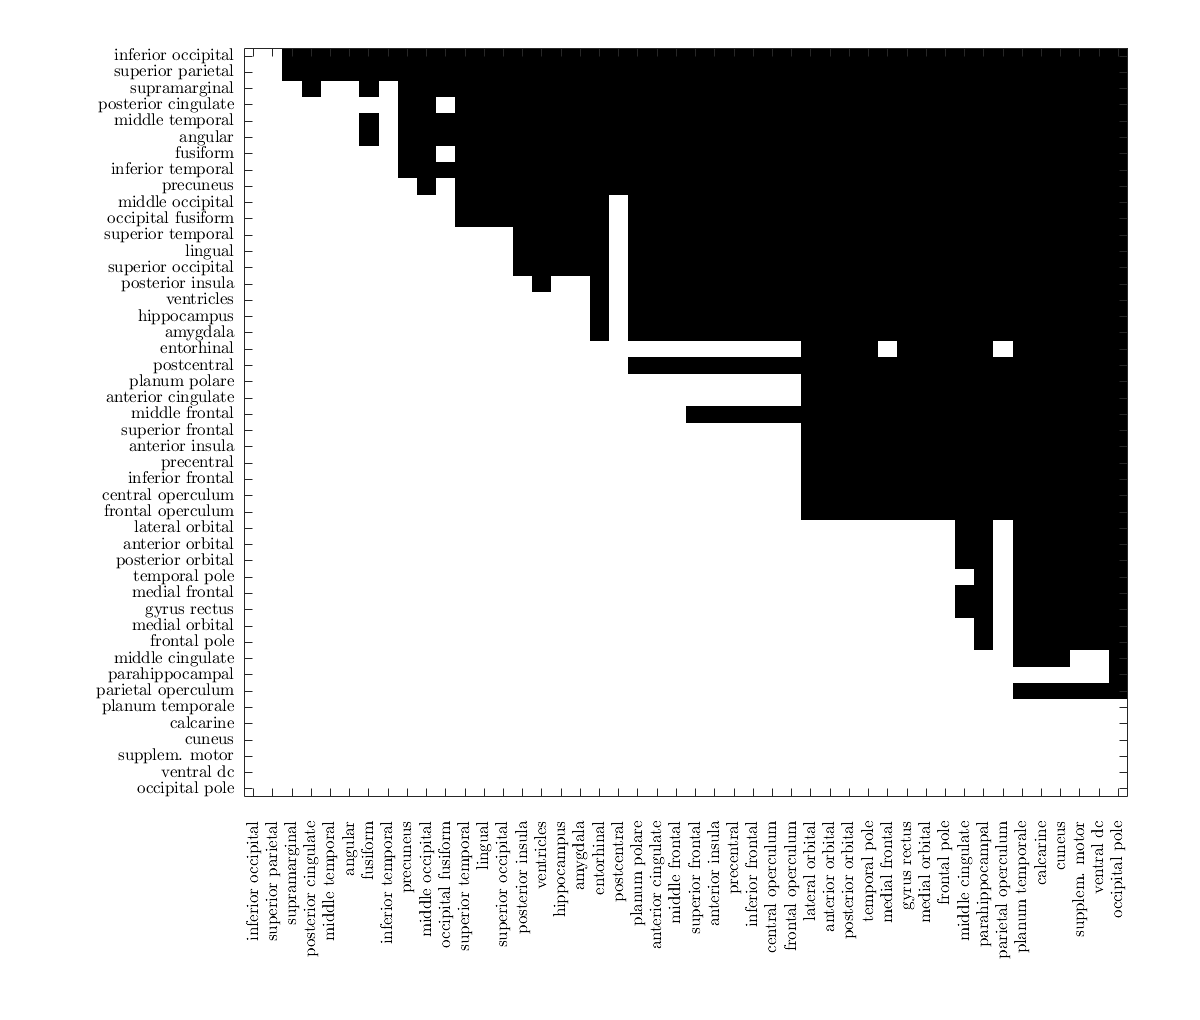
\includegraphics[width=1.2\textwidth,trim=50 30 0 30,clip]{\pcaPaperFigs/statTestSPA.png}
 \end{subfigure}

\begin{subfigure}[t]{0.48\textwidth}
\centering
   \textbf{\large{\mbox{Object perception impairment group}}}
 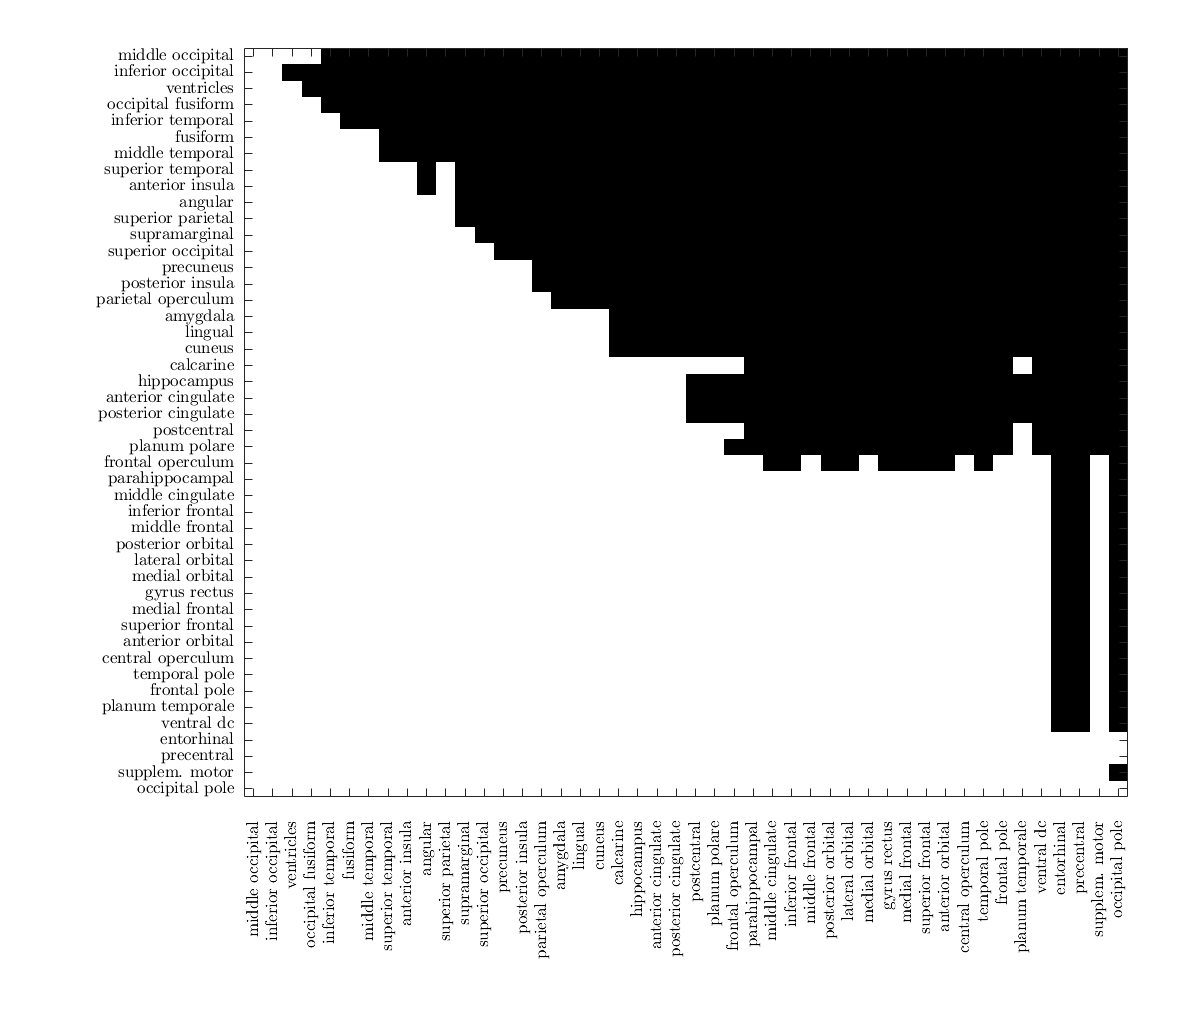
\includegraphics[width=1.2\textwidth,trim=50 30 0 30,clip,valign=t]{\pcaPaperFigs/statTestPER.png}
 \end{subfigure}
 \caption[Hypothesis testing of the ordering of events within the three PCA subgroups.]{Hypothesis testing of the ordering of events within the three PCA subgroups. Hypothesis tests were designed as in \ref{fig:statTestPcaAd}}
\label{fig:statTestEarSpaPer}
\end{figure}

\FloatBarrier


 % PCA T = -10 

\begin{table}
\centering
\begin{tabular}{c |c c c c c c c c }
Region & Whole Br. & Ventricles & Hippo. & Entorh. & Occipital & Temporal & Frontal & Parietal\\
\hline 
Whole Brain & - & - & - & - & - & - & - & -\\
Ventricles & 1.74e-04* & - & - & - & - & - & - & -\\
Hippo. & 1.20e-02 & 4.95e-02 & - & - & - & - & - & -\\
Entorhinal & 1.61e-12* & 1.27e-06* & 5.29e-10* & - & - & - & - & -\\
Occipital & 7.93e-03 & 4.16e-06* & 1.20e-04* & 9.44e-12* & - & - & - & -\\
Temporal & 2.66e-01 & 1.17e-02 & 3.12e-01 & 5.90e-10* & 1.81e-03 & - & - & -\\
Frontal & 9.58e-01 & 1.57e-04* & 1.07e-02 & 1.52e-12* & 8.68e-03 & 2.49e-01 & - & -\\
Parietal & 3.45e-04* & 1.31e-08* & 2.52e-07* & 3.17e-15* & 8.84e-01 & 7.91e-05* & 4.08e-04* & -\\
\end{tabular} 
\caption[Statistical testing for significant differences in volumes of different brain regions of PCA subjects at -10 years before$t_0$]{Statistical testing for significant differences in volumes of different brain regions of PCA subjects at -10 years before reference $t_0$. Shown here are p-values from two-tailed t-tests. (*) Statistically significant differences at significance level = 1.78e-3, Bonferroni corrected for all 28 comparisons. } 
\label{tab:demStatTestVolsPcaMinus10}
\end{table}



% PCA T = 0 

\begin{table}
\centering
\begin{tabular}{c |c c c c c c c c }
Region & Whole Br. & Ventricles & Hippo. & Entorh. & Occipital & Temporal & Frontal & Parietal\\
\hline 
Whole Brain & - & - & - & - & - & - & - & -\\
Ventricles & 1.52e-16* & - & - & - & - & - & - & -\\
Hippo. & 6.03e-13* & 8.95e-06* & - & - & - & - & - & -\\
Entorhinal & 4.78e-14* & 5.66e-01 & 9.60e-04* & - & - & - & - & -\\
Occipital & 1.32e-06* & 3.17e-17* & 1.45e-14* & 5.25e-16* & - & - & - & -\\
Temporal & 3.57e-01 & 1.75e-16* & 5.22e-13* & 2.90e-14* & 1.66e-05* & - & - & -\\
Frontal & 7.31e-12* & 1.67e-04* & 7.72e-01 & 4.38e-03 & 1.62e-14* & 3.50e-12* & - & -\\
Parietal & 1.53e-07* & 1.41e-21* & 3.30e-19* & 2.68e-19* & 2.20e-01 & 8.33e-06* & 3.39e-18* & -\\


\end{tabular} 
\caption[Statistical testing for significant differences in volumes of different brain regions of PCA subjects at $t_0$]{Statistical testing for significant differences in volumes of different brain regions of PCA subjects at $t_0$. See Supp. Table \ref{tab:demStatTestVolsPcaMinus10} for information on statistical testing.} 
\label{tab:demStatTestVolsPca0}
\end{table}

 % PCA T = 10 

\begin{table}
\centering
\begin{tabular}{c |c c c c c c c c }
Region & Whole Br. & Ventricles & Hippo. & Entorh. & Occipital & Temporal & Frontal & Parietal\\
\hline 
Whole Brain & - & - & - & - & - & - & - & -\\
Ventricles & 5.97e-01 & - & - & - & - & - & - & -\\
Hippo. & 7.63e-13* & 4.14e-13* & - & - & - & - & - & -\\
Entorhinal & 5.88e-11* & 2.34e-11* & 1.23e-03* & - & - & - & - & -\\
Occipital & 4.04e-02 & 1.44e-01 & 3.00e-17* & 1.06e-15* & - & - & - & -\\
Temporal & 2.83e-03 & 1.22e-02 & 1.51e-15* & 2.66e-14* & 1.54e-01 & - & - & -\\
Frontal & 8.90e-15* & 5.73e-15* & 6.77e-02 & 7.35e-07* & 2.19e-19* & 2.99e-17* & - & -\\
Parietal & 7.38e-02 & 2.07e-01 & 1.25e-14* & 4.00e-13* & 9.44e-01 & 1.73e-01 & 1.91e-16* & -\\


\end{tabular} 
\caption[Statistical testing for significant differences in volumes of different brain regions of PCA subjects at 10 years after $t_0$.]{Statistical testing for significant differences in volumes of different brain regions of PCA subjects at 10 years after $t_0$. See Supp. Table \ref{tab:demStatTestVolsPcaMinus10} for information on statistical testing.} 
\label{tab:demStatTestVolsPcaPlus10}
\end{table}


 % AD T = -10 

\begin{table}
\centering
\begin{tabular}{c |c c c c c c c c }
Region & Whole Br. & Ventricles & Hippo. & Entorh. & Occipital & Temporal & Frontal & Parietal\\
\hline 
Whole Brain & - & - & - & - & - & - & - & -\\
Ventricles & 9.26e-03 & - & - & - & - & - & - & -\\
Hippo. & 2.04e-10* & 2.88e-14* & - & - & - & - & - & -\\
Entorhinal & 2.21e-02 & 3.40e-01 & 6.82e-09* & - & - & - & - & -\\
Occipital & 3.38e-03 & 2.01e-06* & 3.84e-04* & 9.98e-04* & - & - & - & -\\
Temporal & 3.93e-01 & 1.04e-01 & 4.72e-11* & 7.64e-02 & 7.51e-04* & - & - & -\\
Frontal & 8.30e-01 & 1.04e-02 & 4.79e-09* & 2.41e-02 & 1.15e-02 & 3.26e-01 & - & -\\
Parietal & 4.94e-03 & 2.13e-06* & 3.75e-05* & 4.63e-04* & 7.35e-01 & 8.64e-04* & 1.57e-02 & -\\

\end{tabular} 
\caption[Statistical testing for significant differences in volumes of different brain regions of tAD subjects at -10 years before $t_0$.]{Statistical testing for significant differences in volumes of different brain regions of tAD subjects at -10 years before $t_0$. See Supp. Table \ref{tab:demStatTestVolsPcaMinus10} for information on statistical testing.} 
\label{tab:demStatTestVolsAdMinus10}
\end{table}

 % AD T = 0 

\begin{table}
\centering
\begin{tabular}{c |c c c c c c c c }
Region & Whole Br. & Ventricles & Hippo. & Entorh. & Occipital & Temporal & Frontal & Parietal\\
\hline 
Whole Brain & - & - & - & - & - & - & - & -\\
Ventricles & 3.50e-11* & - & - & - & - & - & - & -\\
Hippo. & 4.12e-19* & 3.61e-25* & - & - & - & - & - & -\\
Entorhinal & 7.83e-02 & 2.64e-10* & 2.93e-13* & - & - & - & - & -\\
Occipital & 7.65e-02 & 2.51e-08* & 7.95e-10* & 7.94e-01 & - & - & - & -\\
Temporal & 6.29e-03 & 4.63e-13* & 1.84e-14* & 5.12e-01 & 8.07e-01 & - & - & -\\
Frontal & 2.01e-04* & 2.65e-04* & 4.16e-20* & 2.84e-05* & 1.98e-04* & 3.31e-07* & - & -\\
Parietal & 3.56e-03 & 6.00e-11* & 1.94e-10* & 2.45e-01 & 4.77e-01 & 4.81e-01 & 2.12e-06* & -\\
\end{tabular} 
\caption[Statistical testing for significant differences in volumes of different brain regions of tAD subjects at $t_0$.]{Statistical testing for significant differences in volumes of different brain regions of tAD subjects at $t_0$. See Supp. Table \ref{tab:demStatTestVolsPcaMinus10} for information on statistical testing.} 
\label{tab:demStatTestVolsAd0}
\end{table}

 % AD T = 10 

\begin{table}
\centering
\begin{tabular}{c |c c c c c c c c }
Region & Whole Br. & Ventricles & Hippo. & Entorh. & Occipital & Temporal & Frontal & Parietal\\
\hline 
Whole Brain & - & - & - & - & - & - & - & -\\
Ventricles & 2.92e-02 & - & - & - & - & - & - & -\\
Hippo. & 2.83e-01 & 1.67e-03* & - & - & - & - & - & -\\
Entorhinal & 8.13e-03 & 6.50e-01 & 2.63e-04* & - & - & - & - & -\\
Occipital & 8.40e-02 & 9.92e-01 & 1.13e-02 & 7.28e-01 & - & - & - & -\\
Temporal & 2.76e-12* & 1.46e-14* & 5.41e-11* & 6.35e-15* & 2.54e-10* & - & - & -\\
Frontal & 1.24e-09* & 1.91e-06* & 3.87e-11* & 4.81e-06* & 1.27e-04* & 2.43e-19* & - & -\\
Parietal & 7.92e-01 & 7.53e-02 & 1.98e-01 & 2.51e-02 & 1.57e-01 & 5.36e-11* & 3.13e-08* & -\\
\end{tabular} 
\caption[Statistical testing for significant differences in volumes of different brain regions of tAD subjects at 10 years after $t_0$.]{Statistical testing for significant differences in volumes of different brain regions of tAD subjects at 10 years after $t_0$. See Supp. Table \ref{tab:demStatTestVolsPcaMinus10} for information on statistical testing.} 
\label{tab:demStatTestVolsPlus10}
\end{table}


\begin{table}
\centering
\begin{tabular}{c |c c c }
Region & T1 = -10 years &  T2 = 0 years &  T3 = 10 years\\
\hline
Whole Brain & 2.52e-02 & 4.45e-05* & 4.19e-12*\\
Ventricles & 3.74e-05* & 3.06e-05* & 2.18e-13*\\
Hippocampus & 6.15e-15* & 1.13e-23* & 5.83e-04*\\
Entorhinal & 5.28e-08* & 7.71e-11* & 2.68e-03\\
Occipital & 5.72e-01 & 1.13e-05* & 2.44e-12*\\
Temporal & 2.48e-02 & 1.21e-02 & 4.02e-11*\\
Frontal & 2.91e-02 & 6.26e-03 & 2.12e-01\\
Parietal & 4.22e-01 & 2.95e-07* & 8.33e-12*\\

\end{tabular}
\caption[Statistical testing for significant differences in volumes of different brain regions between PCA and tAD at -10, 0 and 10 years from $t_0$.]{Statistical testing for significant differences in volumes of different brain regions between PCA and tAD at -10, 0 and 10 years from $t_0$. Shown here are p-values from two-tailed t-tests. (*) Statistically significant differences at significance level = 2.08e-3, Bonferroni corrected for all 28 comparisons.}
\label{tab:demStatTestPcaAd}
\end{table}


\begin{figure}
% \vspace{-8em}
 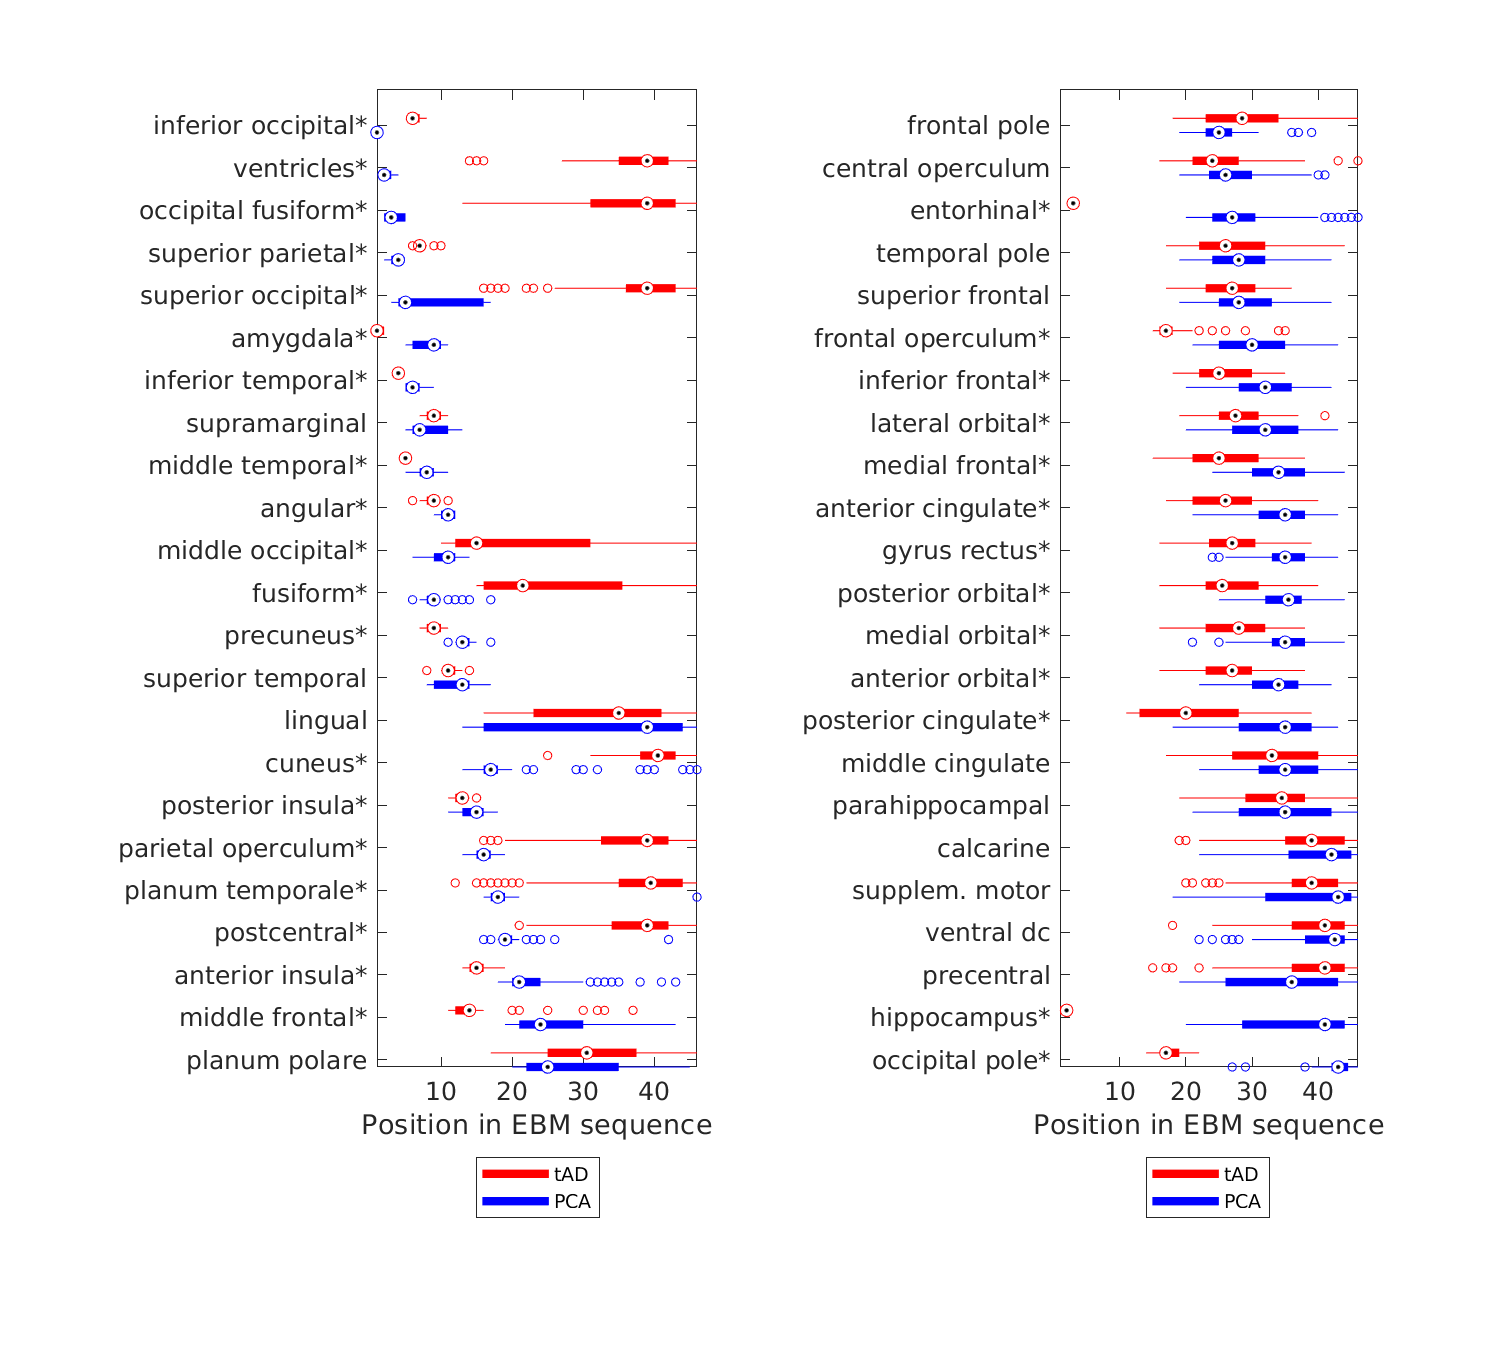
\includegraphics[width=\textwidth,trim=50 50 50 0,clip]{\pcaPaperFigs/statTestTwoDis_PCA_AD}
 \caption[Testing for statistically significant differences in positions of each biomarker in the EBM abnormality sequences, for both PCA and typical AD.]{Testing for statistically significant differences in positions of each biomarker in the EBM abnormality sequences, for both PCA and typical AD. (*) Statistically significant differences in position of a biomarker in the EBM sequences for PCA and tAD at 99\% confidence, Bonferroni corrected for multiple comparisons (significance level = 5e-5). A non-parametric Mann-Whitney U test has been applied because of non-gaussianity of the data, which represents discrete ranks in a sequence. Most biomarkers show significant differences -- it is likely that there are differences in atrophy progression between PCA and tAD.}
 \label{fig:ebmStatTestPcaAd}
\end{figure}


\begin{figure}
%  \centering
\begin{subfigure}{\textwidth}
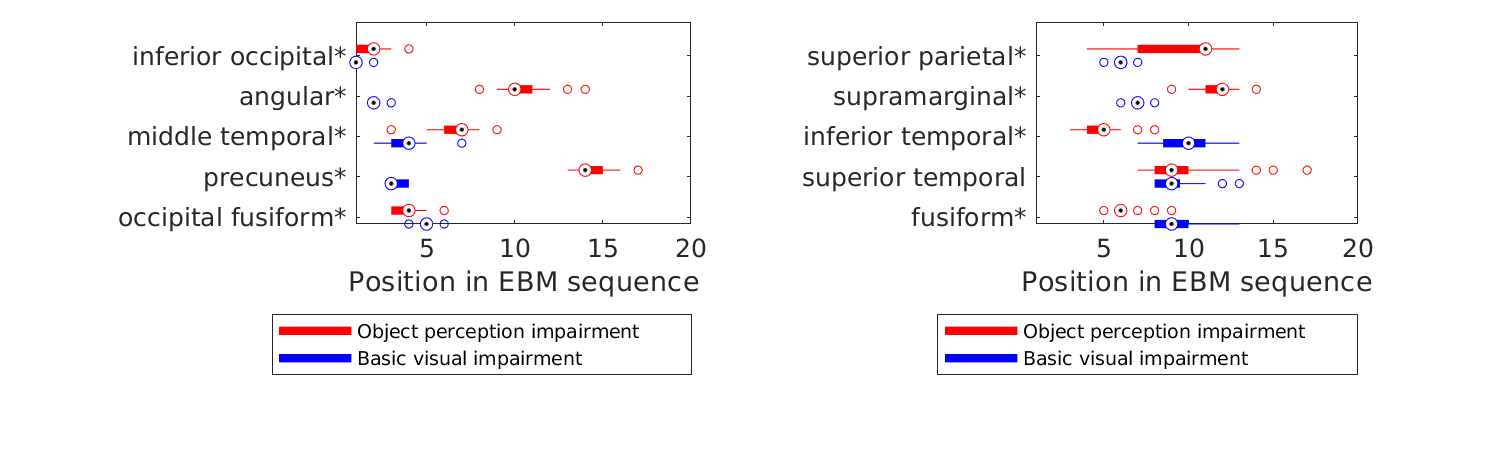
\includegraphics[width=1\textwidth,trim=0 20 0 0,clip]{\pcaPaperFigs/statTestTwoDis_EAR_PER}
\caption{Vision vs Object subgroups}
\end{subfigure}

\begin{subfigure}{\textwidth}
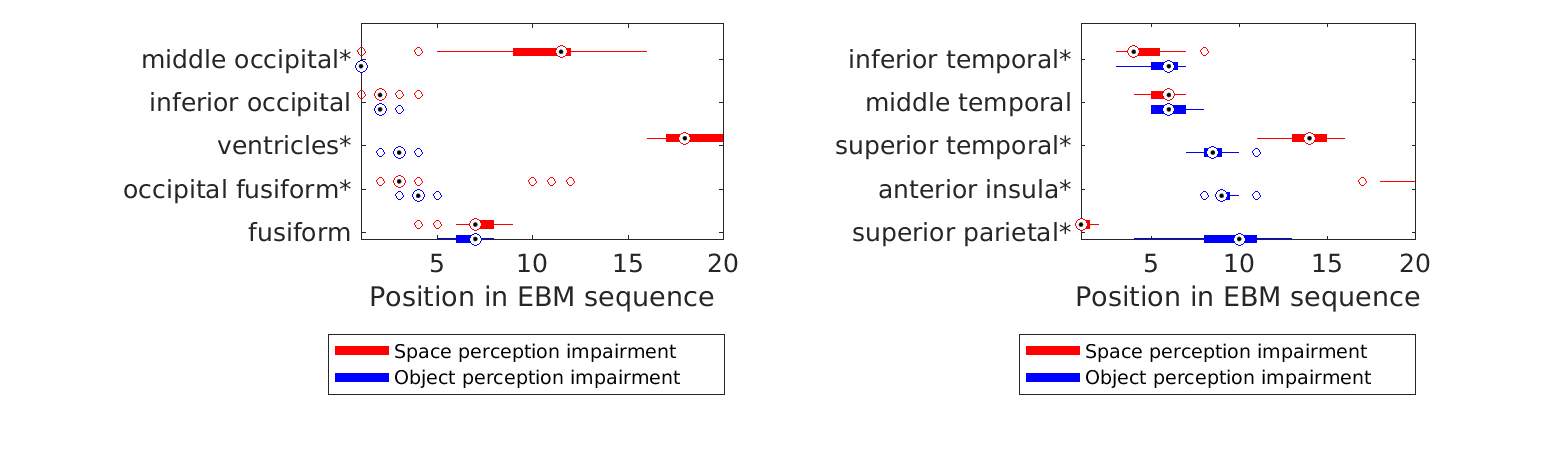
\includegraphics[width=1\textwidth,trim=0 20 0 0,clip]{\pcaPaperFigs/statTestTwoDis_PER_SPA}
\caption{Object vs Space subgroups}
\end{subfigure}


\begin{subfigure}{\textwidth}
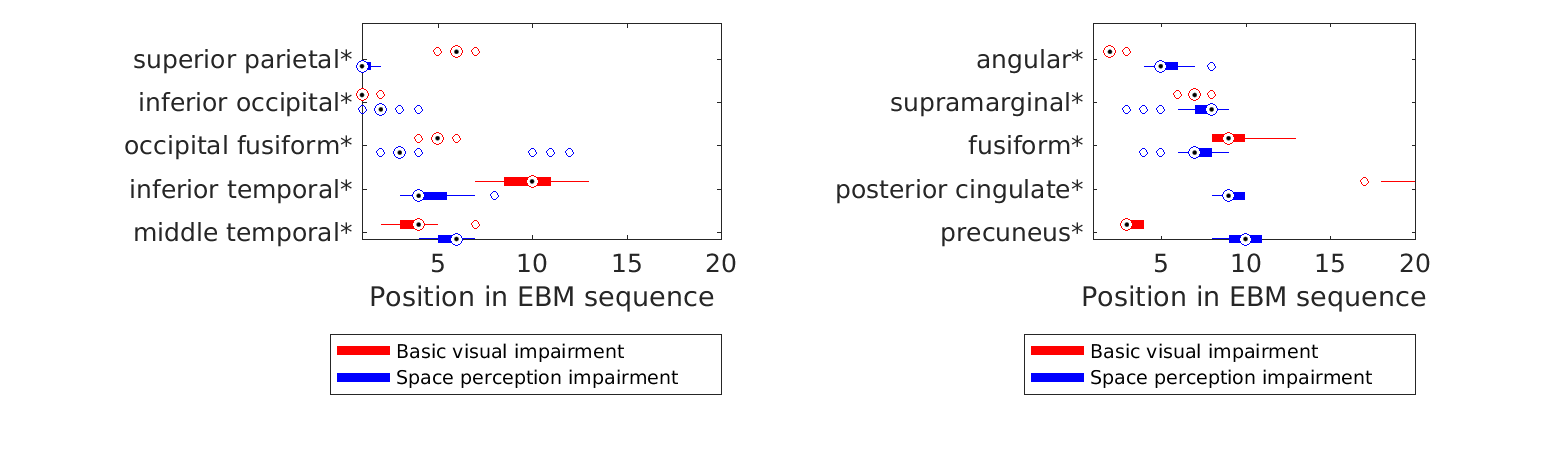
\includegraphics[width=1\textwidth,trim=0 20 0 0,clip]{\pcaPaperFigs/statTestTwoDis_SPA_EAR}
\caption{Space vs Vision subgroups}
\end{subfigure}

\caption[Testing for statistically significant differences in biomarker positions in the EBM sequences of PCA subgroups.]{Testing for statistically significant differences in biomarker positions in the EBM sequences of PCA subgroups for (a) Object vs Visual (b) Space vs Object and (c) Visual vs Space subgroups.  Only the first 10 biomarkers from the EBM sequence of one disease (A -- visual B -- object C -- space) are shown. The images also show only the first 20 positions on the x-axis to aid visualisation. (*) Statistically significant differences in biomarker positions between pairs of PCA subgroups at 99\% confidence, Bonferroni corrected for multiple comparisons (significance level = 5e-5). A non-parametric Mann-Whitney U test has again been applied because of data non-gaussianity. All biomarkers show significant differences -- it is likely that there are differences in the progression of atrophy between PCA subgroups.}
\label{fig:ebmStatTestPcaSubgroups}
\end{figure}



\chapter[DIVE: A Spatiotemporal Progression Model of Brain Pathology]{DIVE: A Spatiotemporal Progression Model of Brain Pathology in Neurodegenerative Disorders}
\label{sec:diveAppendix}

\def\ci{\perp\!\!\!\perp}

\clearpage

\section{Simulations - Error in Estimated Trajectories and DPS}

\begin{figure}[H]
\begin{picture}(230,180)
\put(0,0){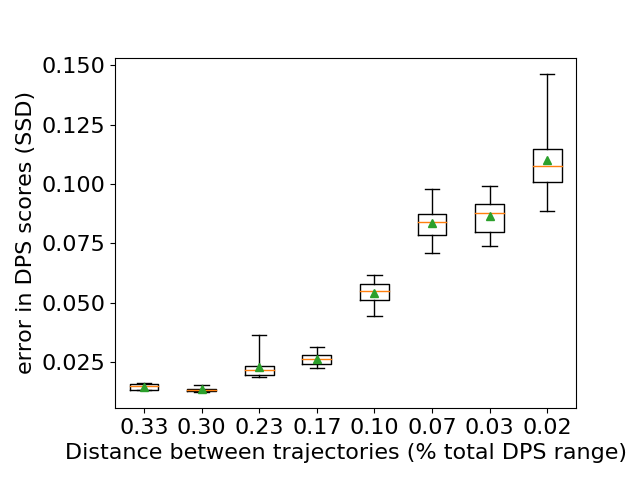
\includegraphics[width=0.45\textwidth]{\voxDpmFolder/resfiles/synth/dpsError_trajCent.png}}
\put(30,160){\textbf{\huge{A}}}
\end{picture} 
\begin{picture}(230,180)
\put(0,0){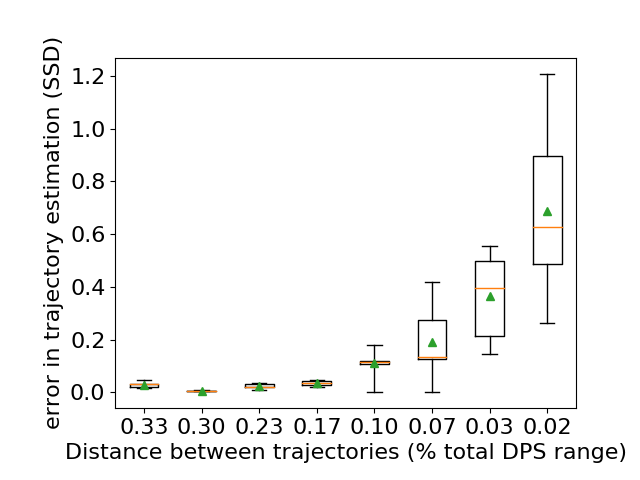
\includegraphics[width=0.45\textwidth]{\voxDpmFolder/resfiles/synth/thetaError_trajCent.png}}
\put(30,160){\textbf{\huge{B}}}
\end{picture} 

\begin{picture}(230,180)
\put(0,0){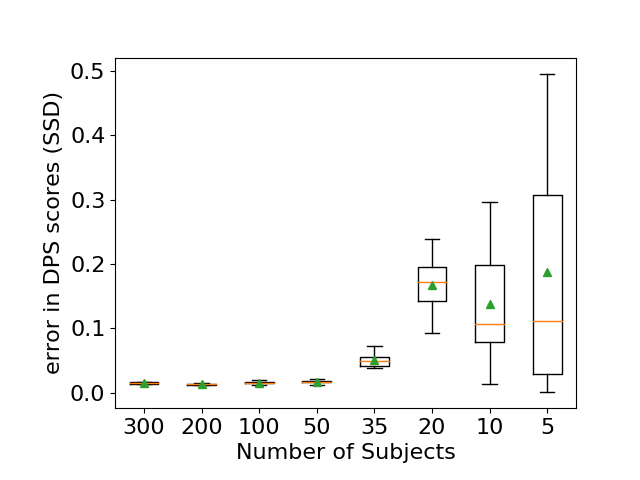
\includegraphics[width=0.45\textwidth]{\voxDpmFolder/resfiles/synth/dpsError_nrSubj.png}}
\put(30,160){\textbf{\huge{C}}}
\end{picture} 
\begin{picture}(230,180)
\put(0,0){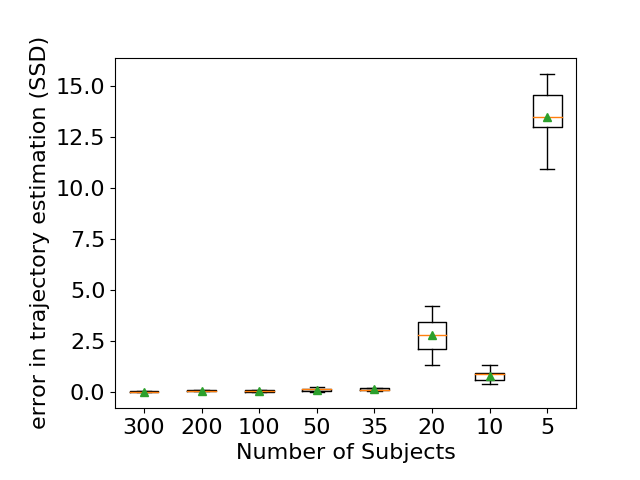
\includegraphics[width=0.45\textwidth]{\voxDpmFolder/resfiles/synth/thetaError_nrSubj.png}}
\put(30,160){\textbf{\huge{D}}}
\end{picture} 
\caption[DIVE: Error in DPS scores and trajectory estimation in simulations]{Error in DPS scores (A) and trajectory estimation (B) for Scenario 2 in simulation experiments. (C-D) The same error scores for Scenario 3. We notice that as the problem becomes more difficult, the errors in the DIVE estimated parameters increase. Errors were measured as sum of squared differences (SSD) between the true parameters and estimated parameters. For the trajectories, the SSD was calculated only based on the sigmoid centres, due to different scaling of the other sigmoidal parameters.}
\label{diveTrajError}
\end{figure}


\section{Comparison Between DIVE and Other Models}
\label{sec:diveCompAppendix}
 
\subsection{Motivation}

We were also interested to compare the performance of DIVE with other disease progression models. In particular, we were interested to test whether:
\begin{itemize}
 \item Modelling dynamic clusters on the brain surface improves subject staging and biomarker prediction
 \item Modelling subject-specific stages with a linear transformation (the $\alpha_i$ and $\beta_i$ terms) improves biomarker prediction
\end{itemize}


\subsection{Experiment Design}

We compared the performance of our model to two simplified models:
\begin{itemize}
 \item ROI-based model: groups vertices according to an a-priori defined ROI atlas. This model is equivalent to the model by Jedynak et al., Neuroimage, 2012 and is a special case of our model, where the latent variables $z_{lk}$ are fixed instead of being marginalised as in equation 6.
 \item No-staging model: This is a model that doesn't perform any time-shift of patients along the disease progression timeline. It fixes $\alpha_i=1$, $\beta_i=0$ for every subject, which means that the disease progression score of every subject is age.
\end{itemize}

We performed this comparison using 10-fold cross-validation. For each subject in the test set, we computed their DPS score and correlated all the DPS values with the same four cognitive tests used previously. We also tested how well the models can predict the future vertex-wise measurements as follows: for every subject i in the test set, we used their first two scans to estimate $\alpha_i=1$, $\beta_i=0$ and then used the rest of the scans to compute the prediction error. For one vertex location on the cortical surface, the prediction error was computed as the root mean squared error (RMSE) between its predicted measure and the actual measure. This was then averaged across all subjects and visits. 


\subsection{Results}

Table \ref{tab1} shows the results of the model comparison, on ADNI MRI dataset. Each row represents one model tested, while each column represents a different performance measure: correlations with four different cognitive tests and accuracy in the prediction of future vertexwise measurements. In each entry, we give the mean and standard deviation of the correlation coefficients or RMSE across the 10 cross-validation folds.  

\begin{table}[H]
\centering
\begin{footnotesize}
 \begin{tabular}{c | c c c c | c}
  Model & CDRSOB ($\rho$) & ADAS13 ($\rho$) & MMSE ($\rho$) & RAVLT ($\rho$) & Prediction (RMSE)\\
  \hline 
%   DIVE & 0.37 +/- 0.10 & 0.37 +/- 0.09 & -0.37 +/- 0.11 & -0.32 +/- 0.12 & 1.00 +/- 0.01\\
%   ROI-based model & 0.41 +/- 0.11 & 0.41 +/- 0.10 & -0.41 +/- 0.11 & -0.35 +/- 0.11 & 1.00 +/- 0.01\\
%   No-staging model & 0.03 +/- 0.14 & -0.02 +/- 0.13 & 0.02 +/- 0.12 & -0.01 +/- 0.12 & 1.05 +/- 0.02\\
DIVE & 0.37 +/- 0.09 & 0.37 +/- 0.10 & 0.36 +/- 0.11 & 0.32 +/- 0.12 & 1.021 +/- 0.008 \\
ROI-based model & 0.36 +/- 0.10 & 0.35 +/- 0.11 & 0.34 +/- 0.13 & 0.30 +/- 0.13 & 1.019 +/- 0.010 \\
No-staging model & *0.09 +/- 0.06 & *0.03 +/- 0.09 & *0.05 +/- 0.06 & *0.02 +/- 0.06 & *1.062 +/- 0.024 \\

 \end{tabular}
 \end{footnotesize}
 \caption[Comparison of DIVE with two more simplistic models on the ADNI MRI dataset.]{Comparison of DIVE with two more simplistic models on the ADNI MRI dataset. For each of the three models, we show the correlation of the disease progression scores (DPS) with respect to several cognitive tests: CDRSOB, ADAS13, MMSE and RAVLT. The correlation numbers represent the mean correlation across the 10 cross-validation folds. }
 \label{tab1}
\end{table}



\section{Derivation of the Generalised EM Algorithm}
\label{sec:diveEmDerivAppendix}

We seek to calculate $M^{(u)} = \argmax_{M} \mathbb{E}_{Z|V,M^{(u-1)}} \left[log\ p(V,Z|M)\right] + log\ p(M)$  where $M^{(u)} = (\alpha^{(u)}, \beta^{(u)}, \theta^{(u)}, \sigma^{(u)}, \lambda^{(u)})$ are the set of model parameters at iteration $u$ of the EM algorithm. Moreover, $p(M^{(u)})$ is a prior on these parameters that is chosen by the user. Expanding the expected value, we get:

\begin{equation}
\label{eq:EM1}
M^{(u)} = \argmax_{M} \sum_{z1,\dots, z_L}^K p(Z = (z_1, ..., z_L) | V, \Mu^{(u-1)}) \left[log\ p(V,Z|M)\right] + log\ p(M) 
\end{equation}


The E-step involves computing $p\left(Z = (z_1, ..., z_L)| V, \Mu^{(u-1)}\right)$, while the M-step comprises of solving the above equation. 


\subsection{E-step}

In this step we need to estimate $p(Z | V, \Mu^{(u-1)})$. For notational simplificy we will drop the $(u-1)$ superscript from $\Mu$

\begin{equation}
 p(Z | V, \Mu) = \frac{1}{C}  p(V, Z | \Mu) =  \prod_l^L \left[ \prod_{(i,j) \in I} N(V_l^{ij} | f(\alpha_i t_{ij} + \beta_i | \theta_{Z_l}), \sigma_{Z_l})  \prod_{l_2 \in N_l} \Psi (Z_{l}, Z_{l_2}) \right]
\end{equation}
where $N_l$ is the set of neighbours of vertex $l$. However, this doesn't directly factorise over the vertices $l$ due to the MRF terms $\Psi (Z_{l}, Z_{l_2})$. It is however necessary to find a form that factorises over the vertices, otherwise we won't be able to represent in memory the joint distribution over all $Z$ variables. If we make the approximation $p(Z | V, \Mu) \approx \prod_l^L p(V_l|Z_l, \Mu)$ then we loose out all the MRF terms and the model won't account for spatial correlation. We instead do a first-degree approximation by conditioning on the values of $Z_{N_l}^{(u-1)}$, the labels of nearby vertices from the previous iteration. The approximation is thus:

\begin{equation}
\label{eq:app_e_approx}
 p(Z | V, \Mu) \approx \prod_l^L \mathbb{E}_{Z_{N_l}^{(u-1)}|V_l, M} \left[ p(Z_l|V_l, \Mu, Z_{N_l}^{(u-1)}) \right]
\end{equation}

This form allows us to factorise over all the vertices to get $p(Z_l | V_l, \Mu)$:

\begin{equation}
 p(Z_l | V_l, \Mu) \approx \frac{1}{C} \sum_{Z_{N_l}^{(u-1)}} p(V_l|Z_l, \Mu) p(Z_l|Z_{N_l}^{(u-1)}) p(Z_{N_l}^{(u-1)}|V_l, M) 
\end{equation}

where $C$ is a normalistion constant that can be dropped. We can now  further factorise $p(Z_l|Z_{N_l}^{(u-1)}) \approx  \prod_{m \in \{1, ..., N_l\}} p(Z_l | \Mu,  Z_{N_l(m)}^{(u-1)} = z_{N_l(m)})$ and apply a similar factorisation to the prior $p(Z_{N_l}^{(u-1)}|V_l, M) $, resulting in:

\begin{multline}
 p(Z_l | V_l, \Mu) \approx \frac{1}{C} p(V_l|Z_l, \Mu) \sum_{z_{N_l(1)}, .., z_{N_l(|N_l|)}}\ \ \  \prod_{m \in \{1, ..., N_l\}} p(Z_l | Z_{N_l(m)}^{(u-1)} = z_{N_l(m)}) \\ p(Z_{N_l(m)}^{(u-1)} = z_{N_l(m)}|V_l, M)
\end{multline}


Factorising the summation over $z_{N_l}$'s we get:

\begin{equation}
 p(Z_l | V_l, \Mu) = p(V_l| Z_l, \Mu)   \prod_{l_2 \in N_l} \sum_{z_{l_2}} p(Z_l | Z_{l_2}^{(u-1)} = z_{l_2}) p(Z_{l_2}^{(u-1)} = z_{l_2}|V_l, M)
\end{equation}

Replacing $z_{l_2}$ with $k_2$ we get:

\begin{equation}
 p(Z_l | V_l, \Mu) = p(V_l| Z_l, \Mu)   \prod_{l_2 \in N_l} \sum_{k_2} p(Z_l | Z_{l_2}^{(u-1)} = k_2) p(Z_{l_2}^{(u-1)} = k_2|V_l, M)
\end{equation}


We shall also denote $z_{lk} = p(Z_l | V_l, \Mu)$. Further simplifications result in:
%We will denote this as  $z_{lk} = p(Z_l = k | V, \Mu^{(u-1)})$.

\begin{equation}
 z_{lk}^{(u)} \propto  \left[ \prod_{i,j \in I} N(V_l^{ij} | f(\alpha_i t_{ij} + \beta_i | \theta_k), \sigma_k) \right] \left[ \prod_{l_2 \in N_l} \sum_{k_2 = 1}^K z_{l_2k_2}^{(u-1)}\ \Psi (Z_{l} = k, Z_{l_2} = k_2) \right]
\end{equation}


\begin{multline}
 log\ z_{lk}^{(u)} \propto  \left[ \sum_{i,j \in I} -\frac{log\ (2 \pi \sigma_k^2)}{2} - \frac{1}{2\sigma_k^2}(V_l^{ij} - f(\alpha_i t_{ij} + \beta_i | \theta_k))^2 \right] + \\ + \left[\sum_{l_2 \in N_l} log \sum_{k_2 = 1}^K z_{l_2k_2}^{(u-1)} (\delta_{k_2 k}\ exp(\lambda) + (1 - \delta_{k_2 k})\ exp(-\lambda^2)) \right]
\end{multline}


We further define the data-fit term $D_{lk}$ as follows:
\begin{equation}
\label{eq:app_e-step_Dlk}
D_{lk} = -\frac{log\ (2 \pi \sigma_k^2) |I|}{2} - \sum_{i,j \in I}  \frac{1}{2\sigma_k^2}(V_l^{ij} - f(\alpha_i t_{ij} + \beta_i | \theta_k))^2 
\end{equation}


This results in:

\small
\begin{equation}
 log\ z_{lk}^{(u)} \propto  D_{lk} + \left[\sum_{l_2 \in N_l} log \sum_{k_2 = 1}^K z_{l_2k_2}^{(u-1)} (\delta_{k_2 k}\ (exp(\lambda) - exp(-\lambda^2)) + exp(-\lambda^2)) \right]
\end{equation}
\normalsize


Finally, we simplify the sum over $k_2$ to get the update equation for $z_{lk}$:

% \small
\begin{equation}
\label{eq:app_e-step}
\begin{split}
 log\ z_{lk}^{(u)} \propto D_{lk}+ \left[ \sum_{l_2 \in N_l} log\ \left[ exp(-\lambda^2) + z_{l_2k}^{(u-1)} (exp(\lambda) - exp(-\lambda^2)) \right] \right]
\end{split}
\end{equation}
% \normalsize

In practice, we cannot naively compute the exponential term $z_{lk} = exp(log(z_{lk}))$ due to precision loss. However, we go around this by recomputing the exponentiation and normalisation of $z_{lk}$ simultaneously. Denoting $x(k) = log\ z_{lk}$, for  $k \in [1 \dots K]$, we get: 

\begin{equation}
 z_{lk}  = \frac{e^{x(k)}}{e^{x(1)}+e^{x(2)} + \dots + e^{x(K)}} = \frac{1}{e^{x(1)-x(k)} +e^{x(2)-x(k)} + \dots + e^{x(K)-x(k)}}
\end{equation}



\subsection{M-step}

The M-step itself does not have a closed-form analytical solution. We choose to solve it by successive refinements of the cluster trajectory parameters and the subject time shifts. 

\subsection{Optimising Trajectory Parameters}


\textbf{Trajectory shape - $\theta$}\\

Taking equation \ref{eq:EM1} and fixing the subject time-shifts $\alpha$, $\beta$ and measurement noise $\sigma$, we can find its maximum with respect to $\theta$ only. More precisely, we want:

\begin{equation}
 \theta = \argmax_{\theta} \sum_{z1,\dots, z_L}^K p(Z = (z_1, ..., z_L) | V, \Mu^{(u-1)}) \left[ log\ p(V,Z|M) \right] + log\ p(\theta)
\end{equation}

We observe that for each cluster the individual $\theta_k$'s are conditionally independent, i.e. $\theta_k \ci \theta_m | \{Z, \alpha, \beta, \sigma$\} $\forall k,m$. We also assume that the prior factorizes for each $\theta_k$: $\log p(\theta) = \prod_k^K \log p(\theta_k)$. This allows us to optimise each $\theta_k$ independently:

\begin{equation}
 \theta_k = \argmax_{\theta_k} \sum_{z1,\dots, z_L}^K p(Z = (z_1, ..., z_L) | V, \Mu^{(u-1)}) \left[ log\ p(V,Z|M) \right] + log\ p(\theta_k)
\end{equation}

Replacing the full data log-likelihood, we get:

\begin{multline}
 \theta_k = \argmax_{\theta_k} \sum_{z1,\dots, z_L}^K p(Z = (z_1, ..., z_L) | V, \Mu^{(u-1)})\ \\ log \left[ \prod_{l=1}^L \prod_{(i,j) \in I} N(V_l^{ij} | f(\alpha_i t_{ij} + \beta_i | \theta_{z_l}), \sigma_{z_l}) \right]  + log\ p(\theta_k)
\end{multline}

Note that we didn't include the MRF clique terms, since they are not a function of $\theta_k$. We propagate the logarithm inside the products:

\begin{multline}
 \theta_k = \argmax_{\theta_k} \sum_{z1,\dots, z_L}^K p(Z = (z_1, ..., z_L) | V, \Mu^{(u-1)}) \sum_{l=1}^L \sum_{(i,j) \in I} log\ N(V_l^{ij} | f(\alpha_i t_{ij} + \beta_i | \theta_{z_l}), \sigma_{z_l}) + \\ + log\ p(\theta_k)
\end{multline}

\begin{sloppypar}
We next assume that $Z_l$, the hidden cluster assignment for vertex $l$, is conditionally independent of the other vertex assignments $Z_m$, $\forall m \neq l$ (See E-step approximation from Eq. \ref{eq:app_e_approx}). This independence assumption induces the following factorization: ${p(Z = (z_1, ..., z_L) | V, \Mu^{(u-1)}) = \prod_l^L p(Z_l = z_l | V, \Mu^{(u-1)})}$. Propagating this product inside the sum over the vertices, we get:
\end{sloppypar}


\begin{equation}
\label{eq:SupTheta5}
 \theta_k = \argmax_{\theta_k} \sum_{l=1}^L \sum_{z_l = 1}^K p(Z_l = z_l | V, \Mu^{(u-1)}) \sum_{(i,j) \in I} log\ N(V_l^{ij} | f(\alpha_i t_{ij} + \beta_i | \theta_{z_l}), \sigma_{z_l}) + log\ p(\theta_k)
\end{equation}

The terms which don't contain $\theta_k$ dissapear:

\begin{equation}
 \theta_k = \argmax_{\theta_k} \sum_{l=1}^L p(Z_l = k | V, \Mu^{(u-1)}) \sum_{(i,j) \in I} log\ N(V_l^{ij} | f(\alpha_i t_{ij} + \beta_i | \theta_k), \sigma_k) + log\ p(\theta_k)
\end{equation}

We further expand the Gaussian noise model:

\begin{multline}
 \theta_k = \argmax_{\theta_k} \sum_{l=1}^L p(Z_l = k | V, \Mu^{(u-1)}) \\ \sum_{(i,j) \in I} \left[ log\ (2 \pi \sigma_k)^{-1/2} - \frac{1}{2\sigma_k^2}(V_l^{ij} - f(\alpha_i t_{ij} + \beta_i | \theta_k))^2 \right] + log\ p(\theta_k)
\end{multline}

Constants dissapear due to the $\argmax$ and we get the final update equation for $\theta_k$:

\begin{equation}
 \theta_k = \argmax_{\theta_k} \sum_{l=1}^L p(Z_l = k | V, \Mu^{(u-1)}) \sum_{(i,j) \in I} \left[ - \frac{1}{2\sigma_k^2}(V_l^{ij} - f(\alpha_i t_{ij} + \beta_i | \theta_k))^2 \right] + log\ p(\theta_k)
\end{equation}

\textbf{Measurement noise - $\sigma$}\\

We first assume a uniform prior on the $\sigma$ parameters to simplify derivations. Using a similar approach as with $\theta$, after propagating the product inside the logarithm and removing the terms which don't contain $\sigma_k$, we get:

\begin{equation}
 \sigma_k = \argmax_{\sigma_k} \sum_{l=1}^L p(Z_l = k | V, \Mu^{(u-1)}) \sum_{(i,j) \in I} log\ N(V_l^{ij} | f(\alpha_i t_{ij} + \beta_i | \theta_k), \sigma_k)
\end{equation}

Note that, just as for $\theta$ above, the MRF clique terms were not included because they are not a function of $\sigma_k$. Expanding the noise model we get:

\begin{equation}
 \sigma_k = \argmax_{\sigma_k} \sum_{l=1}^L p(Z_l = k | V, \Mu^{(u-1)}) \sum_{(i,j) \in I} \left[ log\ (2 \pi \sigma_k^2)^{-1/2} - \frac{1}{2\sigma_k^2}(V_l^{ij} - f(\alpha_i t_{ij} + \beta_i | \theta_k))^2 \right]
\end{equation}

The maximum of a function $l(\sigma_k)$ can be computed by taking the derivative of the function $l$ and setting it to zero. This is under the assumption that $l$ is differentiable, which it is but we won't prove it here. This gives:

\begin{equation}
 \frac{\delta l(\sigma_k|.)}{\delta \sigma_k} =  \sum_{l=1}^L p(Z_l = k | V, \Mu^{(u-1)}) \sum_{(i,j) \in I} \frac{\delta}{\delta \sigma_k} \left[ log\ (2 \pi \sigma_k^2)^{-1/2} - \frac{1}{2\sigma_k^2}(V_l^{ij} - f(\alpha_i t_{ij} + \beta_i | \theta_k))^2 \right]
\end{equation}

Propagating the differential operator further inside the sums we get:

\begin{equation}
 \frac{\delta l(\sigma_k|.)}{\delta \sigma_k} =  \sum_{l=1}^L p(Z_l = k | V, \Mu^{(u-1)}) \sum_{(i,j) \in I} \left[ -\frac{\delta}{\delta \sigma_k} \frac{log\ \sigma_k^2}{2} - \frac{\delta}{\delta \sigma_k} \frac{1}{2\sigma_k^2}(V_l^{ij} - f(\alpha_i t_{ij} + \beta_i | \theta_k))^2 \right]
\end{equation}

We next perform several small manipulations to reach a more suitable form of the derivative and then set it to be equal to zero:

\begin{equation}
 \frac{\delta l(\sigma_k|.)}{\delta \sigma_k} =  \sum_{l=1}^L p(Z_l = k | V, \Mu^{(u-1)}) \sum_{(i,j) \in I} \left[ - \frac{1}{\sigma_k} - \frac{-2}{2\sigma_k^3}(V_l^{ij} - f(\alpha_i t_{ij} + \beta_i | \theta_k))^2 \right]
\end{equation}

\begin{equation}
 \frac{\delta l(\sigma_k|.)}{\delta \sigma_k} =  \sum_{l=1}^L p(Z_l = k | V, \Mu^{(u-1)}) \sum_{(i,j) \in I} \left[ - \frac{\sigma_k^2}{\sigma_k^3} + \frac{1}{\sigma_k^3}(V_l^{ij} - f(\alpha_i t_{ij} + \beta_i | \theta_k))^2 \right]
\end{equation}

\begin{equation}
 \frac{\delta l(\sigma_k|.)}{\delta \sigma_k} =  \sum_{l=1}^L p(Z_l = k | V, \Mu^{(u-1)}) \sum_{(i,j) \in I} \left[ - \sigma_k^2 + (V_l^{ij} - f(\alpha_i t_{ij} + \beta_i | \theta_k))^2 \right] = 0
\end{equation}

% \begin{equation}
%  \sum_{l=1}^L p(Z_l = k | V, \Mu^{(u-1)}) \sum_{(i,j) \in I} (V_l^{ij} - f(\alpha_i t_{ij} + \beta_i | \theta_k))^2 = \sum_{l=1}^L p(Z_l = k | V, \Mu^{(u-1)}) \sum_{(i,j) \in I} \sigma_k^2
% \end{equation}

Finally, we solve for $\sigma_k$ and get its update equation: 

\begin{equation}
\label{eq:SupThetaFinal}
 \sigma_k^2 = \frac{1}{|I|} \sum_{l=1}^L p(Z_l = k | V, \Mu^{(u-1)}) \sum_{(i,j) \in I} (V_l^{ij} - f(\alpha_i t_{ij} + \beta_i | \theta_k))^2
\end{equation}

% but I need to correct for DOFs, so:
% 
% \begin{equation}
%  \sigma_k^2 = \frac{1}{|I^{cross}| - 2|I^{long}| - |\theta_k|} \sum_{l=1}^L p(Z_l = k | V, \Mu^{(u-1)}) \sum_{(i,j) \in I} (V_l^{ij} - f(\alpha_i t_{ij} + \beta_i | \theta_k))^2
% \end{equation}


\subsection{Estimating Subject Time Shifts - $\alpha$, $\beta$}

For estimating $\alpha$, $\beta$, we adopt a similar strategy as in the case of $\theta$, up to Eq. \ref{eq:SupTheta5}. This gives us the following problem:

\begin{multline}
 \alpha_i, \beta_i = \argmax_{\alpha_i, \beta_i} \sum_{l=1}^L \sum_{k = 1}^K p(Z_l = k | V, \Mu^{(u-1)}) \sum_{(i',j) \in I} log\ N(V_l^{i'j} | f(\alpha_{i'} t_{i'j} + \beta_{i'} | \theta_{k}), \sigma_{k}) + \\ + log\ p(\alpha_i, \beta_i)
\end{multline}

The terms $\alpha_{i'}, \beta_{i'}$ for other subjects $i' \neq i$ dissappear:

\begin{equation}
 \alpha_i, \beta_i = \argmax_{\alpha_i, \beta_i} \sum_{l=1}^L \sum_{k = 1}^K p(Z_l = k | V, \Mu^{(u-1)}) \sum_{j \in I_i} log\ N(V_l^{ij} | f(\alpha_{i} t_{ij} + \beta_{i} | \theta_{k}), \sigma_{k}) + log\ p(\alpha_i, \beta_i)
\end{equation}

Expanding the Gaussian noise model we get:

\begin{multline}
 \alpha_i, \beta_i = \argmax_{\alpha_i, \beta_i} \sum_{l=1}^L \sum_{k = 1}^K p(Z_l = k | V, \Mu^{(u-1)}) \\ \sum_{j \in I_i} \left[ log\ (2 \pi \sigma_k^2)^{-1/2} - \frac{1}{2\sigma_k^2}(V_l^{ij} - f(\alpha_i t_{ij} + \beta_i | \theta_k))^2 \right] + \ log\ p(\alpha_i, \beta_i)
\end{multline}

After removing constant terms we end up with the final update equation for $\alpha_i$, $\beta_i$:

\begin{multline}
 \alpha_i, \beta_i = \argmin_{\alpha_i, \beta_i}  \left[ \sum_{l=1}^L \sum_{k=1}^K p(Z_l = k | V, \Mu^{(u-1)}) \frac{1}{2\sigma_k^2} \sum_{j \in I_i} (V_l^{ij} - f(\alpha_i t_{ij} + \beta_i | \theta_k))^2\right] - \\ - log\ p(\alpha_i, \beta_i)
\end{multline}

\subsection{Estimating MRF Clique Term - $\lambda$}

We optimise $\lambda$ using the following formula:

\begin{equation}
\lambda^{(u)} = \argmax_{\lambda} E_{p(Z|V, M^{(u-1)}, \lambda, Z^{(u-1)})}[log\ p(V,Z|M^{(u-1)})]
\end{equation}

Note that $p(Z|V, M^{(u-1)}, \lambda, Z^{(u-1)})$ is a function of $\lambda$, so for each lambda we estimate $z_{lk}$ through approximate inference. We do this because otherwise the optimisation of $\lambda$ will only take into account the clique terms and completely exclude the data terms. We further simplify the objective function for lambda as follows:

\begin{multline}
\lambda^{(u)} = \argmax_{\lambda} \sum_{z1,\dots, z_L}^K p(Z = (z_1, ..., z_L) | V, \Mu^{(u-1)}, \lambda, Z^{(u-1)})\ \\ log \left[ \prod_{l=1}^L \prod_{(i,j) \in I} N(V_l^{ij} | f(\alpha_i t_{ij} + \beta_i | \theta_{z_l}), \sigma_{z_l}) \prod_{l = 1}^{L}\prod_{l_2 \in N_l} \Psi (z_{l}, z_{l_2}) \right]
\end{multline}


We take the logarithm:

\begin{multline}
\lambda^{(u)} = \argmax_{\lambda} \sum_{z1,\dots, z_L}^K p(Z = (z_1, ..., z_L) | V, \Mu^{(u-1)}, \lambda, Z^{(u-1)})\ \\ \left[ \sum_{l=1}^L \sum_{(i,j) \in I} log\ N(V_l^{ij} | ..) + \sum_{l = 1}^{L}\sum_{l_2 \in N_l} log\ \Psi (z_{l}, z_{l_2}) \right]
\end{multline}

Let us denote $z_{lk} = p(Z_l = k | V, \Mu^{(u-1)}, \lambda, Z^{(u-1)})$. Assuming independence between the latent variables $Z_l$ we get:

\begin{multline}
\lambda = \argmax_{\lambda} \sum_{l=1}^L \sum_{k=1}^K z_{lk}\ \left[ \sum_{(i,j) \in I} log\ N(V_l^{ij} | ..) \right] + \\ + \sum_{l = 1}^{L} \sum_{k=1}^K z_{lk} \sum_{l_2 \in N_l} \sum_{k_2 = 1}^K z_{l_2k}\ log\ \Psi (Z_{l} = k, Z_{l_2} = k_2)  
\end{multline}

However, we now want to make $z_{lk}$ a function of $\lambda$ as previously mentioned, so $z_{lk}=\zeta_{lk}(\lambda)$, for some function $\zeta_{lk}$. More precisely, using the E-step update from Eq. \ref{eq:app_e-step} we define for each vertex $l$ and cluster $k$ a function $\zeta_{lk}(\lambda)$ as follows:

\begin{equation}
\zeta_{lk}(\lambda) = exp \left( D_{lk} +   \sum_{l_2 \in N_l} log\ \left[ exp(-\lambda^2) + z_{l_2k}^{(u-1)} (exp(\lambda) - exp(-\lambda^2)) \right] \right)
\end{equation}

where $D_{lk}$ is as defined in Eq \ref{eq:app_e-step_Dlk}. We then replace $z_{lk}$ with $\zeta_{lk}(\lambda)$ and introduce the chosen MRF clique model to get:

\begin{equation}
\lambda^{(u)} = \argmax_{\lambda}\ \sum_{l=1}^L \sum_{k=1}^K \zeta_{lk}(\lambda) D_{lk}  + \sum_{l = 1}^{L} \sum_{k}^K \sum_{l_2 \in N_l} \sum_{k_2 = 1}^K \zeta_{lk}(\lambda) \zeta_{l_2k}(\lambda)\ \left[ \delta_{kk_2} \lambda + (1-\delta_{kk_2}) (-\lambda^2)\right]
\end{equation}

We separate the cliques that have matching clusters to the ones that don't:

\begin{equation}
\lambda^{(u)} = \argmax_{\lambda}\ \sum_{l=1}^L \sum_{k=1}^K \zeta_{lk}(\lambda) D_{lk} + \sum_{l = 1}^{L} \sum_{l_2 \in N_l} \sum_{k}^K  \left[ \zeta_{lk}(\lambda) \zeta_{l_2k}(\lambda)\ \lambda + \sum_{k2 \neq k} \zeta_{lk}(\lambda) \zeta_{l_2k}(\lambda) (-\lambda^2)\right]
\end{equation}

We also factorise the clique terms:

\begin{multline}
\lambda^{(u)} = \argmax_{\lambda}\ \sum_{l=1}^L \sum_{k=1}^K \zeta_{lk}(\lambda) D_{lk} + \lambda \sum_{l = 1}^{L} \sum_{l_2 \in N_l} \sum_{k}^K   \zeta_{lk}(\lambda) \zeta_{l_2k}(\lambda)\ + \\ + (-\lambda^2) \sum_{l = 1}^{L} \sum_{l_2 \in N_l} \sum_{k}^K \zeta_{lk}(\lambda) (1- \zeta_{l_2k}(\lambda))
\end{multline}

Finally, we simplify to get the objective function for $\lambda$.

\begin{equation}
 \lambda^{(u)} = \argmax_{\lambda}\ \sum_{l=1}^L \sum_{k=1}^K \zeta_{lk}(\lambda) \left[  D_{lk} \  + \lambda \sum_{l_2 \in N_l}  \zeta_{l_2 k}(\lambda)\  -\lambda^2 \sum_{l_2 \in N_l} (1- \zeta_{l_2 k}(\lambda))  \right]
\end{equation}

For implementation speed-up, data-fit terms $D_{lk}$ can be pre-computed.


\section{Fast DIVE Implementation - Proof of Equivalence}
\label{sec:appDivFas}

Fitting DIVE can be computationally prohibitive, especially given that the number of vertices/voxels can be very high, e.g. more than 160,000 in our datasets. We derived a fast implementtion of DIVE, which is based on the idea that for each subject we compute a weighted mean of the vertices within a particular cluster, and then compare that mean with the corresponding trajectory value. This is in contrast with comparing the value at each vertex with the corresponding trajectory of its cluster. In the next few subsections, we will present the mathematical formulation of the fast implementation for parameters [$\theta$, $\alpha$, $\beta$]. Parameter $\sigma$ already has a closed-form update, while parameter $\lambda$ has a more complex update procedure for which this fast implementation doesn't work. For each parameter, we will also provide proofs of equivalence.

\subsection{Trajectory Parameters - $\theta$}

\subsection{Fast Implementation}

The fast implementation for $\theta$ implies that, instead of optimising Eq. \ref{eq:SupThetaFinal} we optimise the following problem:
\begin{equation}
\label{eq:supThetaFast1}
 \theta_k = \argmin_{\theta_k} \sum_{(i,j) \in I} (<V^{ij}>_{\hat{Z}_k} - f(\alpha_i t_{ij} + \beta_i | \theta_k))^2
\end{equation}

where $<V^{ij}>_{\hat{Z}_k}$ is the mean value of the vertices belonging to cluster $k$. Mathematically, we define $\hat{Z}_k = [z_{1k}\gamma_k,\ z_{2k}\gamma_k,\ \dots,\ z_{Lk}\gamma_k ]$ where  $\gamma_k = (\sum_{l=1}^L z_{lk})^{-1}$ is the normalisation constant. Moreover, we have that ${<V^{ij}>_{\hat{Z}_k} = \sum_{l=1}^L z_{lk} \gamma_k V^{ij}}$. We take the derivative of the likelihood function $l_{fast}$ of the fast implementation (Eq. \ref{eq:supThetaFast1}) with respect to $\theta_k$ and perform several simplifications:
\begin{equation}
\frac{\delta l_{fast}(\theta_k|.)}{\delta \theta_k} = \frac{\delta}{\delta \theta_k} \sum_{(i,j) \in I} \left( \sum_{l=1}^L z_{lk} \gamma_k V^{ij} - f(\alpha_i t_{ij} + \beta_i | \theta_k) \right)^2
\end{equation}

\begin{equation}
\frac{\delta l_{fast}(\theta_k|.)}{\delta \theta_k} = \sum_{(i,j) \in I} 2 \left( \left( \sum_{l=1}^L \gamma_k z_{lk} V^{ij} \right) - f(\alpha_i t_{ij} + \beta_i | \theta_k) \right) \frac{-\delta f(.)}{\delta \theta_k}
\end{equation}

using the fact that $\sum_{l=1}^L \gamma_k z_{lk} = 1$ we get:

\begin{equation}
\frac{\delta l_{fast}(\theta_k|.)}{\delta \theta_k} = \sum_{(i,j) \in I} 2 \left( \sum_{l=1}^L \gamma_k z_{lk} \left( V^{ij} - f(\alpha_i t_{ij} + \beta_i | \theta_k) \right) \right) \frac{-\delta f(.)}{\delta \theta_k}
\end{equation}

\begin{equation}
\frac{\delta l_{fast}(\theta_k|.)}{\delta \theta_k} = 2 \gamma_k \sum_{(i,j) \in I} \frac{-\delta f(.)}{\delta \theta_k} \left( \sum_{l=1}^L z_{lk} \left( V^{ij} - f(\alpha_i t_{ij} + \beta_i | \theta_k) \right) \right)
\end{equation}

By setting the derivative to zero, the optimal $\theta$ is thus a solution of the following equation:

\begin{equation}
\label{eq:supThetaFast2}
\sum_{(i,j) \in I} \frac{-\delta f(.)}{\delta \theta_k} \left( \sum_{l=1}^L z_{lk} \left( V^{ij} - f(\alpha_i t_{ij} + \beta_i | \theta_k) \right) \right) = 0
\end{equation}


\subsection{Slow Implementation}

We will prove that if theta is a solution of the slow implementation, it is also a solution of Eq. \ref{eq:supThetaFast2}, which will prove that the fast implementation is equivalent. The slow implementation is finding $\theta$ from the following equation:

\begin{equation}
 \theta_k = \argmin_{\theta_k} \sum_{l=1}^L z_{lk} \sum_{(i,j) \in I} (V_l^{ij} - f(\alpha_i t_{ij} + \beta_i | \theta_k))^2
\end{equation}

Taking the derivative of the function above ($l_{slow}$) with respect to $\theta_k$ we get:
\begin{equation}
\frac{\delta l_{slow}(\theta_k|.)}{\delta \theta_k} = \sum_{l=1}^L z_{lk} \sum_{(i,j) \in I} 2 (V_l^{ij} - f(\alpha_i t_{ij} + \beta_i | \theta_k)) \left(-\frac{\delta f(.)}{\delta \theta_k} \right) = 0
\end{equation}

After swapping terms around and using distributivity we get:

\begin{equation}
  \sum_{(i,j) \in I} \left(-\frac{\delta f(.)}{\delta \theta_k} \right) \sum_{l=1}^L z_{lk} (V_l^{ij} - f(\alpha_i t_{ij} + \beta_i | \theta_k))  = 0
\end{equation}

This is the same optimisation problem as in Eq. \ref{eq:supThetaFast2}, which proves that the two formulations are equivalent with respect to $\theta$.

\subsection{Noise Parameter - $\sigma$}

The noise parameter $\sigma$ can actually be computed in a closed-form solution for the original slow model implementation, so there is no benefit in implementing the fast update for $\sigma$. Moreover, the $\sigma$ in the fast implementation computed the standard deviation in the \emph{mean value} of the vertices within a certain cluster, and not the deviation withing the \emph{actual value} of the vertices.

\subsection{Subjects-specific Time Shifts - $\alpha$, $\beta$}

\subsection{Fast Implementation}

The equivalent fast formulation for the subject-specific time shifts is similar to the one for the trajectory parameters. It should be noted however that we need to weight the sums corresponding to each cluster by $\gamma_{k}^{-1}$. This gives the following equation for the fast formulation:

\begin{equation}
 \alpha_i, \beta_i = \argmin_{\alpha_i, \beta_i}  \sum_{k=1}^K \gamma_k^{-1} \frac{1}{2\sigma_k^2} \sum_{j \in I_i} (<V_l^{ij}>_{\hat{Z}_k} - f(\alpha_i t_{ij} + \beta_i | \theta_k))^2 = 0
\end{equation}

In order to prove that this is equivalent to the slow version, we need to take the derivative of the likelihood function ($l_{fast}$) from the above equation with respect to $\alpha_i$, $\beta_i$ and set it to zero:

\begin{equation}
 \frac{\delta l_{fast}(\alpha_i, \beta_i|.)}{\delta \alpha_i, \beta_i} =  \frac{\delta}{\delta \alpha_i, \beta_i} \sum_{k=1}^K \gamma_k^{-1} \frac{1}{2\sigma_k^2} \sum_{j \in I_i} (<V_l^{ij}>_{\hat{Z}_k} - f(\alpha_i t_{ij} + \beta_i | \theta_k))^2 = 0
\end{equation}

We expand the average across the vertices and slide the derivative operator inside the sums:

\begin{equation}
 \sum_{k=1}^K \gamma_k^{-1} \frac{1}{2\sigma_k^2} \sum_{j \in I_i} 2 \left( \sum_{l=1}^L \gamma_k z_{lk} V_l^{ij} - f(\alpha_i t_{ij} + \beta_i | \theta_k) \right) \frac{-\delta f(.)}{\delta \alpha_i, \beta_i}
\end{equation}

Since $ \sum_{l=1}^L \gamma_k z_{lk} = 1$ we get:

\begin{equation}
 2 \sum_{k=1}^K \gamma_k^{-1} \frac{1}{2\sigma_k^2} \sum_{j \in I_i} \frac{-\delta f(.)}{\delta \alpha_i, \beta_i}  \left( \sum_{l=1}^L \gamma_k z_{lk} (V_l^{ij} - f(\alpha_i t_{ij} + \beta_i | \theta_k)) \right) 
\end{equation}

Removing the factor 2 and sliding $\gamma_k$:

\begin{equation}
 \sum_{k=1}^K \gamma_k^{-1} \gamma_k \frac{1}{2\sigma_k^2} \sum_{j \in I_i} \frac{-\delta f(.)}{\delta \alpha_i, \beta_i}  \left( \sum_{l=1}^L  z_{lk} (V_l^{ij} - f(\alpha_i t_{ij} + \beta_i | \theta_k)) \right) 
\end{equation}

Further sliding $\sum_{l=1}^L z_{lk}$ to the left we get the final optimisation problem:
\begin{equation}
\label{eq:supAlphaFast2}
 \sum_{k=1}^K  \frac{1}{2\sigma_k^2} \sum_{l=1}^L z_{lk} \sum_{j \in I_i} \frac{- \delta f(.)}{\delta \alpha_i, \beta_i} (V_l^{ij} - f(\alpha_i t_{ij} + \beta_i | \theta_k))
\end{equation}


\subsection{Slow Implementation}

In a similar way to the trajectory parameters, we want to prove that solving the problem from Eq. \ref{eq:supAlphaFast2} (fast implementation) is the same as solving the original slow implementation problem, which is defined as:

\begin{equation}
 \alpha_i, \beta_i = \argmin_{\alpha_i, \beta_i}   \sum_{l=1}^L \sum_{k=1}^K z_{lk} \frac{1}{2\sigma_k^2} \sum_{j \in I_i} (V_l^{ij} - f(\alpha_i t_{ij} + \beta_i | \theta_k))^2
\end{equation}

Taking the derivative of the function above with respect to $\alpha_i, \beta_i$, we get:

\begin{equation}
 \frac{\delta l_{slow}(\alpha_i, \beta_i|.)}{\delta \alpha_i, \beta_i} = \sum_{k=1}^K \frac{1}{2\sigma_k^2} \sum_{l=1}^L z_{lk} \sum_{j \in I_i} \frac{- \delta f(.)}{\delta \alpha_i, \beta_i} (V_l^{ij} - f(\alpha_i t_{ij} + \beta_i | \theta_k))
\end{equation}

This is the same problem as the fast implementation one from Eq. \ref{eq:supAlphaFast2}, thus the fast model is equivalent to the slow model with respect to $\alpha$, $\beta$.



\chapter{Disease Knowledge Transfer across Neurodegenerative Diseases}

% \FloatBarrier

%\begin{figure}[H]
% 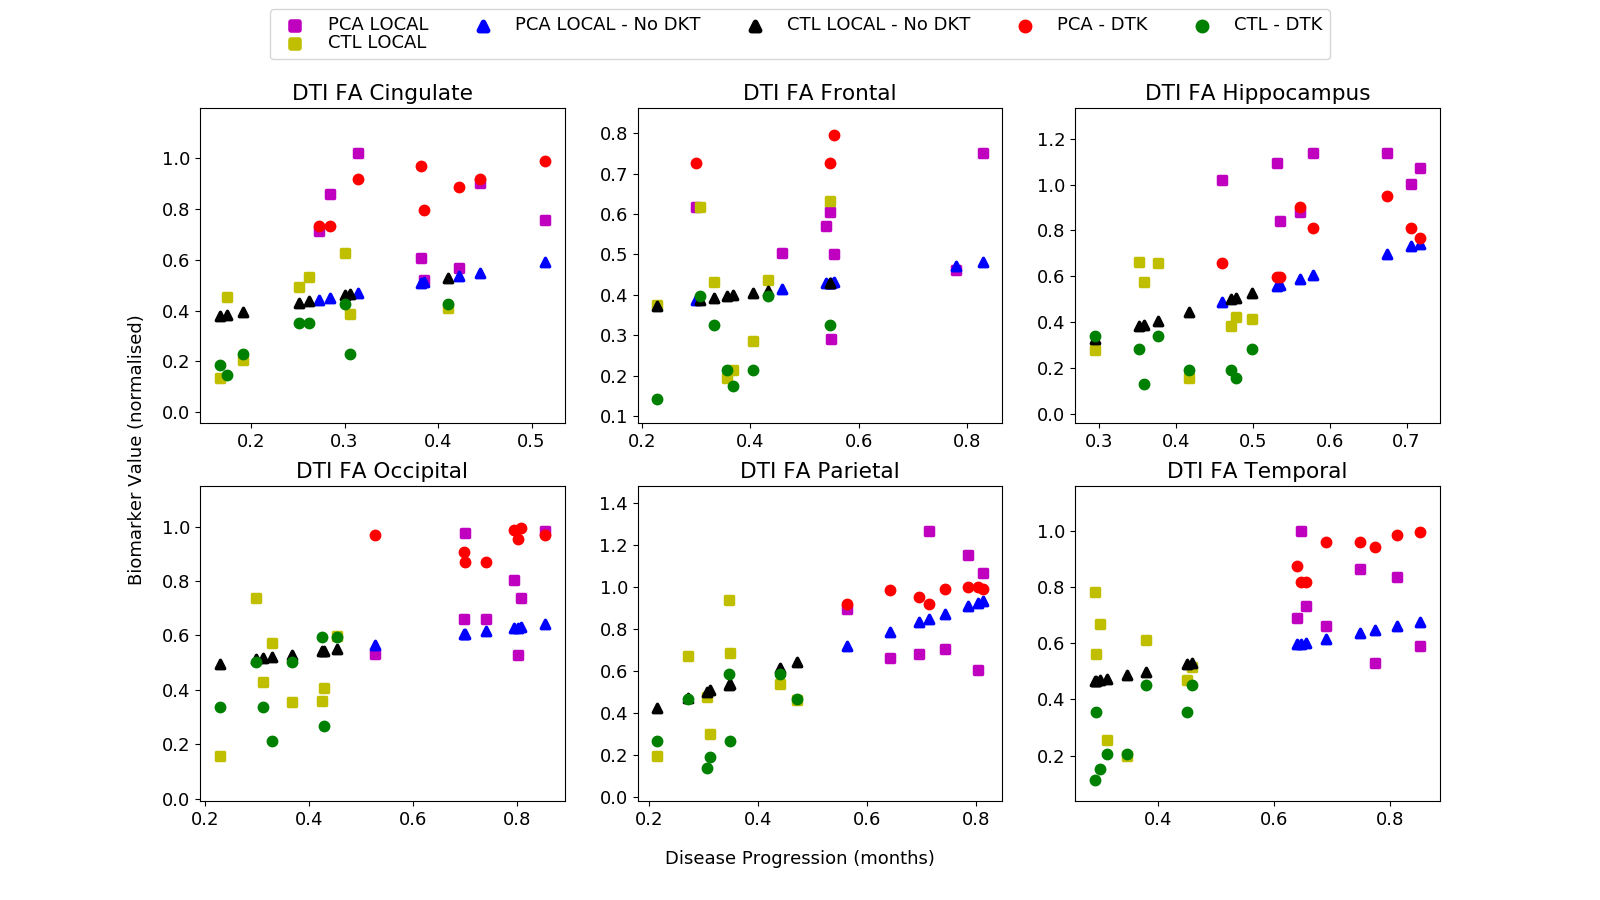
\includegraphics[width=\textwidth, trim=0 0 0 0, clip]{images/dkt/validPredDtiOverMriPCA.png}
% \caption[Validation of the Disease Knowledge Transfer Model using DTI data of PCA subjects from the DRC cohort.]{Validation of the Disease Knowledge Transfer Model using DTI data of PCA subjects from the DRC cohort. Each subject has been shifted along the X-axis only according to their MRI data. No DTI data from PCA subjects was used to fit the model.}
%\label{fig:dktDtiValid}
%\end{figure}


\begin{figure}
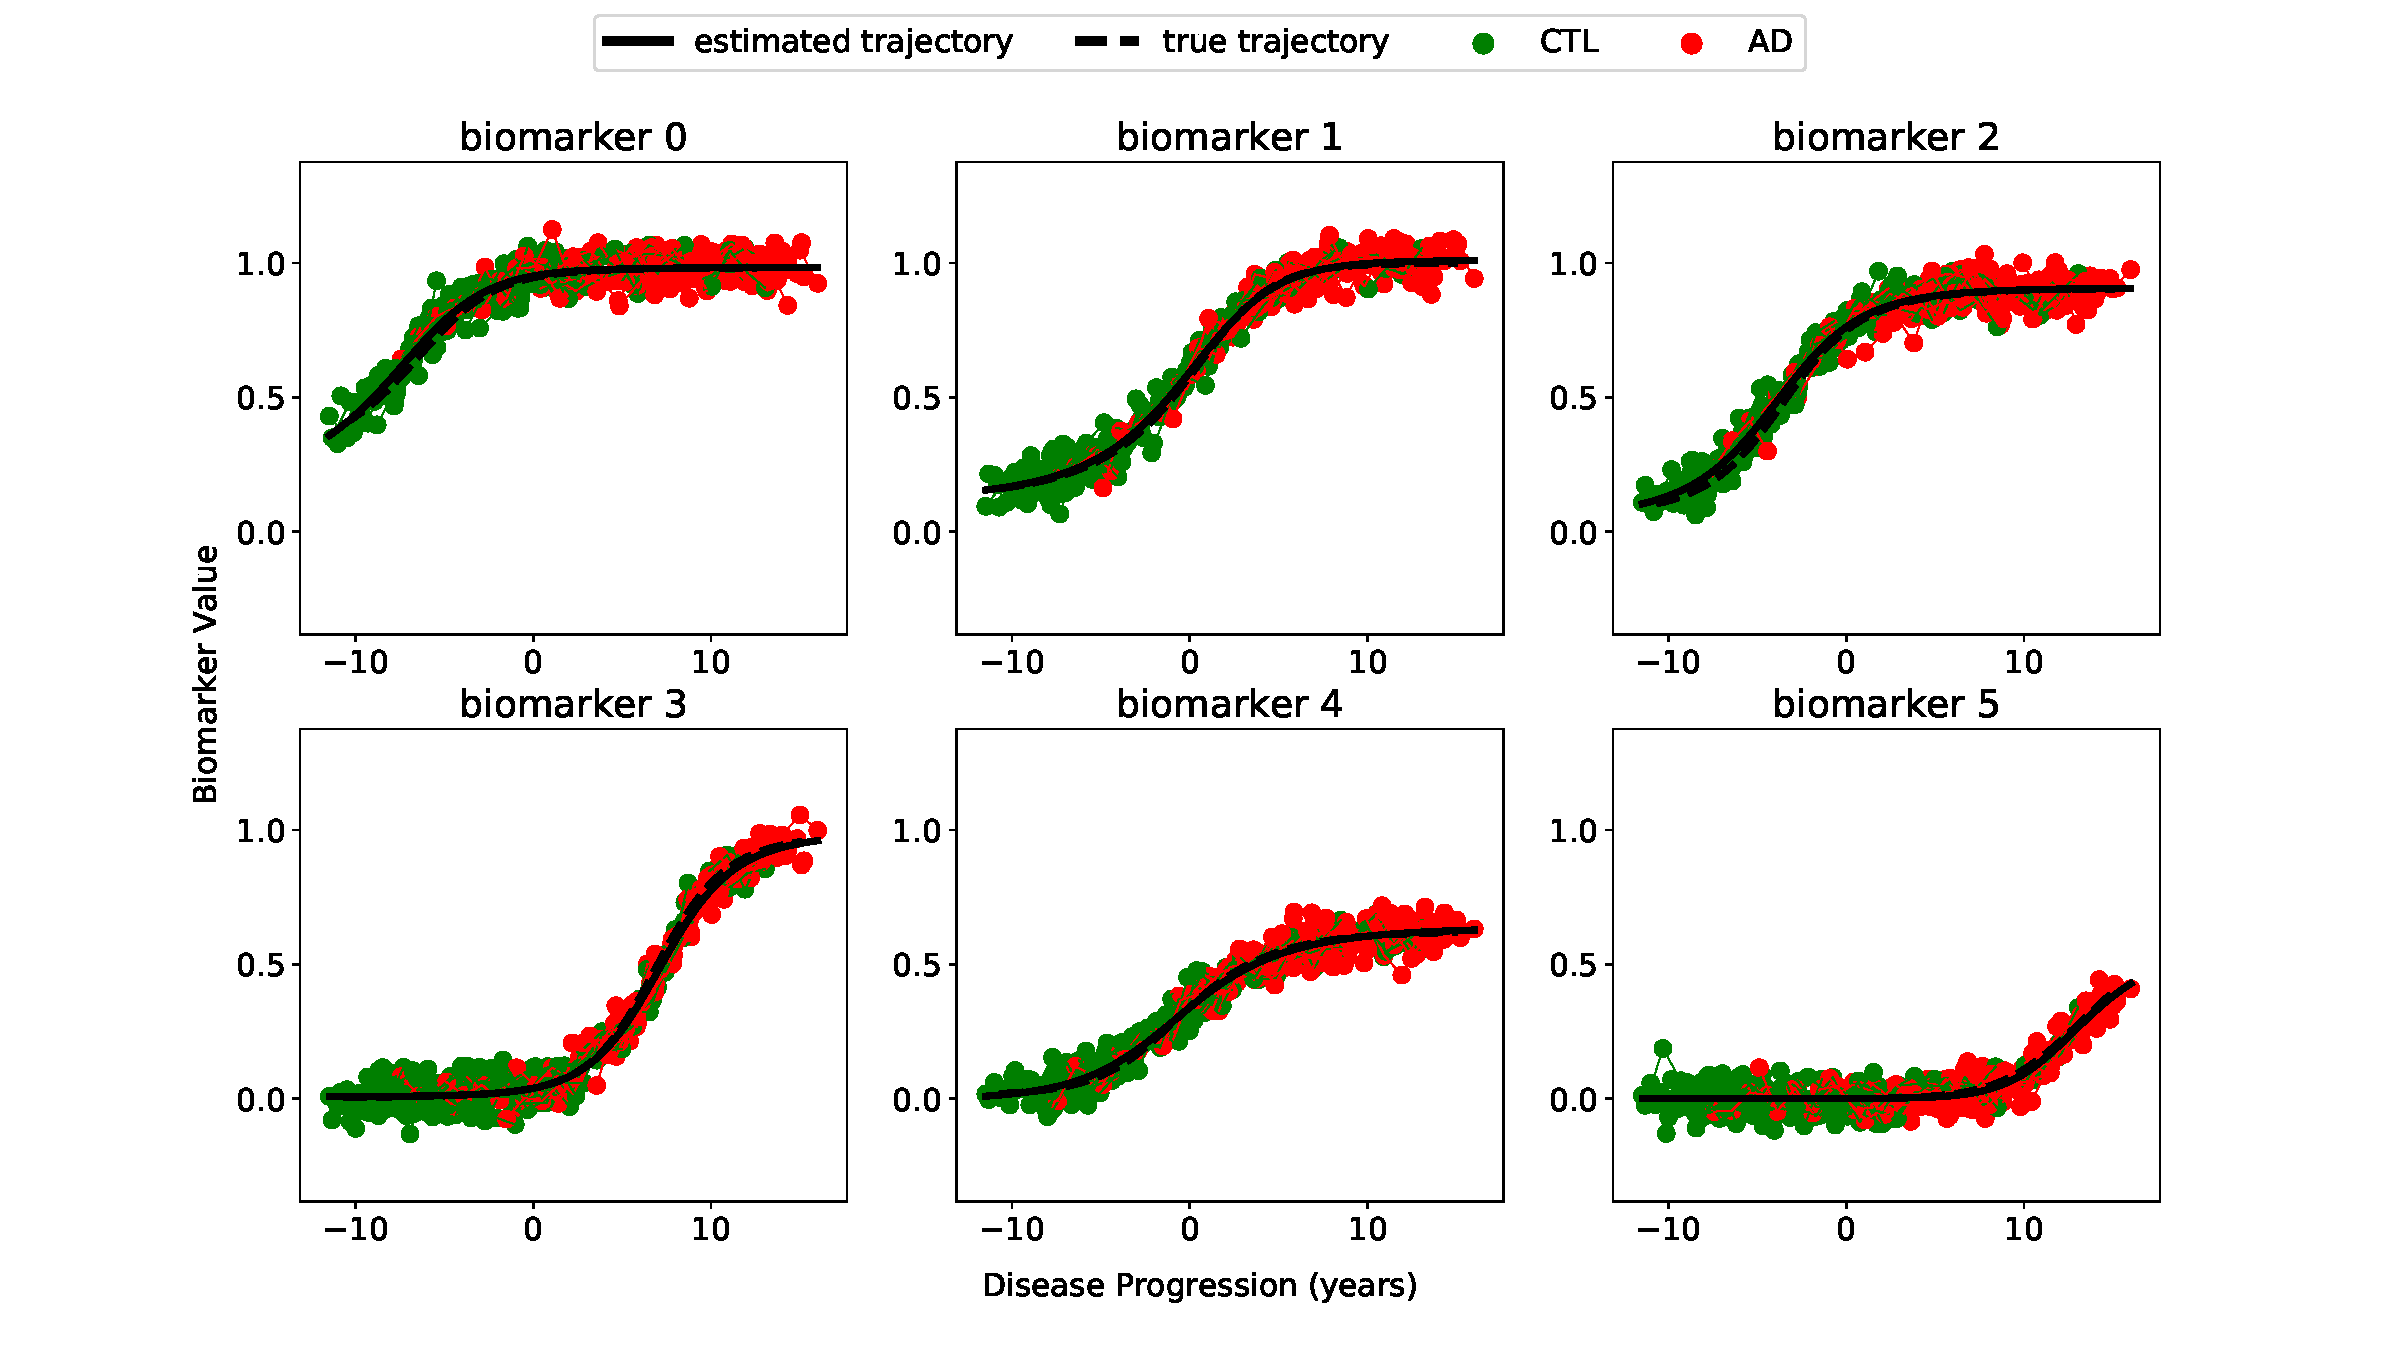
\includegraphics[width=\textwidth]{images/dkt/trajDisSpaceDis0_101_synth1_JMD.pdf}
 \caption[Estimated biomarker trajectories for the "synthetic AD" disease, plotted alongside true trajectories.]{Estimated biomarker trajectories for the "synthetic AD" disease, plotted alongside true trajectories. Estimation of the trajectories in biomarkers 0,1,4 and 5 has been done without any data from the "synthetic PCA" disease, only based on the disease-agnostic correlations with biomarkers 2 and 3.}
 \label{fig:dktSynthTrajADSpace}
\end{figure}

\chapter[Novel Extensions to the EBM and DEM]{Novel Extensions to the Event-based Model and Differential Equation Model}

\section{EBM Fitting using Expectation-Maximisation}
\label{sec:appEbmEm}

Let us assume that $p(x|E)$ and $p(x|\neg E)$ follow normal distributions, where $p(x|E_k) \sim N(\mu^a_k, \sigma^a_k)$ and $p(x|\neg E_k) \sim N(\mu^n_k, \sigma^n_k)$. Our vector of parameters is then given by $\theta = [[\mu_k^n, \sigma_k^n, \mu_k^a, \sigma_k^a]^{k=1..N}, S ]$ where $S$ is the event ordering. Moreover, we further define $Z = [Z_1, Z_2, \dots, Z_P]$ a vector of (latent) discrete random variables representing the stage of each subject which can take values $0 \dots N$, where $N$ is the number of biomarkers. The dataset is denoted by $X$ where $x_{ij}$ represents the data from subject $i$ for biomarker $j$ while $X_i = [x_{i1}, \dots, x_{iN}]$ is a vector of biomarker data for subject $i$. 

\subsection{M-step}

In the M-step we aim to find the arguments $\theta^*$ that maximise the expected log-likelihood of the complete data $\theta^* = \argmax_{\theta} Q(\theta | \theta^{old})$. 

\beq
Q(\theta | \theta^{old}) = \mathbb{E}_{Z|X,\theta^{old}}[log p(X,Z|\theta)]
\eeq

Assuming a uniform prior on $Z$, i.e. $\log p(Z = z) = C$ and expanding $Z$ we get: 
\beq
Q(\theta | \theta^{old}) = C + \sum_{z_1 = 0}^N \dots \sum_{z_P = 0}^N p(Z_1 = z_1, \dots, Z_P = z_P|X, \theta^{old}) log\ p(X|Z_1 = z_1, \dots, Z_P = z_P, \theta)
\eeq

Under the EBM model, the data from each subject is conditionally independent given the parameters, .i.e $X_i \independent X_j|\theta$ and $X_i \independent Z_j|\theta$ for $i \neq j$. A similar independence also holds for the latent variables $Z_i$ given the parameters. We therefore get:
\beq
Q(\theta | \theta^{old}) = C + \sum_{z_1, \dots, z_P} \prod_{i=1}^P  p(Z_i = z_i|X_i, \theta^{old})\ log\left[ \prod_{i=1}^{P} p(X_i|Z_i = z_i, \theta) \right]
\eeq

where $P$ is the number of patients. We further factorise the latent variables $Z$ to obtain:

\beq
Q(\theta | \theta^{old}) = C + \sum_{i=1}^P \sum_{z_i} p(Z_i = z_i|X_i, \theta^{old})\ log\left[ \prod_{i=1}^{P} p(X_i|Z_i = z_i, \theta) \right]
\eeq

After moving the log inside the products and removing the constant $C$ we get:
\beq
Q(\theta | \theta^{old}) = \sum_{i=1}^P \sum_{z_i} p(Z_i = z_i|X_i, \theta^{old}) \left[ \sum_{j=1}^{z_i} log\ p(x_{ij}|E_{S(j)}) + \sum_{j=z_i + 1}^N log\ p(x_{ij}| \neg E_{S(j)}) \right]
\eeq

Replacing $p(x|E)$ and $p(x|\neg E)$ with the pdf of a Gaussian distribution we get:
\begin{multline} 
\label{eq:eStep}
Q(\theta | \theta^{old}) = \sum_{i=1}^P \sum_{z_i}  p(Z_i = z_i|X_i, \theta^{old})\ \sum_{i=1}^{P} \\ \left[ \sum_{j=1}^{z_i} log\ N(x_{ij}|\mu_{S(j)}^a, \sigma_{S(j)}^a) + \sum_{j=z_i + 1}^N log\ N(x_{ij}|\mu_{S(j)}^n, \sigma_{S(j)}^n) \right] \\
\end{multline}

The function $Q(\theta | \theta^{old})$ is differentiable with respect to all parameters apart from $S$ (which is discrete). We can thus find $\theta^*$ by solving $\nabla_{\theta}Q(\theta|\theta_{old}) = 0$. We show the derivation for parameter $\mu_k^n$, which is the solution of  $\frac{d}{d\mu_k^n}Q(\theta | \theta^{old}) = 0 $. Using the result from equation \ref{eq:eStep} and moving the derivation operator inside the sums we get:
\begin{multline}
  \frac{d}{d\mu_k^n}Q(\theta | \theta^{old}) = \sum_{i=1}^P \sum_{z_i}p(Z_i = z_i|X_i, \theta^{old})\ \\ \left[ \sum_{j=1}^{z_i}  \frac{d}{d\mu_k^n}log\ N(x_{ij}|\mu_{S(j)}^a, \sigma_{S(j)}^a) + \sum_{j=z_i + 1}^N \frac{d}{d\mu_k^n}log\ N(x_{ij}|\mu_{S(j)}^n, \sigma_{S(j)}^n) \right] = 0
\end{multline}

The derivative term cancels all likelihood terms apart from the one where $S(j) = k$:

\beq\sum_{i=1}^P \sum_{z_i}p(Z_i = z_i|X_i, \theta^{old})\  \left[ \sum_{j=z_i + 1}^N \mathbb{I}[S(j) = k] \frac{d}{d\mu_k^n}log\ N(x_{ij}|\mu_k^n, \sigma_k^n) \right] = 0
\eeq
which can be rewritten as:
\beq \sum_{i=1}^P \sum_{z_i}p(Z_i = z_i|X_i, \theta^{old})\  \left[ \frac{d}{d\mu_k^n}log\ N(x_{ik}|\mu_k^n, \sigma_k^n) \sum_{j=z_i + 1}^N \mathbb{I}[j = S^{-1}(k)] \right] = 0
\eeq
\beq \sum_{i=1}^P \sum_{z_i} p(Z_i = z_i|X_i, \theta^{old})\  \left[ \frac{d}{d\mu_k^n}log\ N(x_{ik}|\mu_k^n, \sigma_k^n) \mathbb{I}[S^{-1}(k) > z_i] \right] = 0
\eeq
Further rearranging the sum terms we get:

\beq \sum_{i=1}^{P} \frac{d}{d\mu_k^n}log\ N(x_{ik}|\mu_k^n, \sigma_k^n) \sum_{z_i = 0}^N \mathbb{I}[S^{-1}(k) > z_i]\ p(Z_i = z_i | X, \theta^{old})\ = 0
\eeq

\beq \sum_{i=1}^{P} \frac{d}{d\mu_k^n}log\ N(x_{ik}|\mu_k^n, \sigma_k^n) \ p(S^{-1}(k) > Z_i | X, \theta^{old})\ = 0
\eeq
Inserting the formula for the Gaussian pdf we get:
\beq \sum_{i=1}^{P} \frac{d}{d\mu_k^n}\frac{(x_{ik} - \mu_k^n)^2}{2(\sigma_k^n)^2} \ p(S^{-1}(k) > Z_i | X, \theta^{old})\ = 0
\eeq
which results in the update rule for $\mu_k^n$, the mean of $p(x|\neg E_k)$
\beq \mu_k^n = \sum_{i=1}^P x_{ik} w_i^n\eeq\\
where
\beq 
w_i^n = \frac{p(S^{-1}(k) > Z_i | X, \theta^{old})}{\sum_{i=1}^P \ p(S^{-1}(k) > Z_i | X, \theta^{old})}
\eeq
and
\beq
p(S^{-1}(k) > Z_i | X, \theta^{old}) = \sum_{l=S^{-1}(k)+1}^{K} p(Z_i = l | X, \theta^{old})
\eeq
Using a similar approach we get the update rules for $\sigma_k^n$, $\mu_k^a$, $\sigma_k^a$:
\beq \sigma_k^n = \sqrt{\sum_{i=1}^P w_i^n (x_{ik} - \mu_k^n)^2} \eeq \\
\beq \mu_k^a = \sum_{i=1}^P x_{ik} w_i^a \eeq\\
\beq \sigma_k^a = \sqrt{\sum_{i=1}^P w_i^a (x_{ik} - \mu_k^a)^2} \eeq \\
where
\beq w_i^a = \frac{p(S^{-1}(k) \leq Z_i | X, \theta^{old})}{\sum_{i=1}^P \ p(S^{-1}(k) \leq Z_i | X, \theta^{old})}\eeq


Solving for $S$ in the M-step is intractable, so we use MCMC sampling where at each step of the sampling process we propose a new sequence $S^{new}$, find the optimal distribution parameters for each biomarker given $S^{new}$ using the EM update rules and then evaluate the likelihood $Q(\theta | \theta^{old})$. The sequence and parameters that maximise the likelihood are chosen and the EM proceeds to a new iteration. Although this approach might not guarantee that we truly find the optimal parameters, it still results in an increase of $Q(\theta | \theta^{old})$. This approach, called generalised EM, still guarantees that the method will still converge to a local maxima \cite{bishop2007pattern}. For parameter initialisation, we use the mean and standard deviation of the control and patient populations. 

\subsection{E-step}

In the E-step, we simply estimate the latent disease stages $Z_i$ for every subject $i$. The probability $p(Z_i = l|X, \theta^{old})$ that subject $i$ is at stage $l$ in the abnormality sequence, conditioned on the previous parameters $\theta^{old}$, has a closed-form solution given by:

\begin{equation}
p(Z_i = l|X, \theta^{old}) = \frac{\prod_{j=1}^{l} N(x_{i,s(j)}|\mu_{S(j)}^a, \sigma_{S(j)}^a)\prod_{j=l + 1}^N log\ N(x_{i,s(j)}|\mu_{S(j)}^n, \sigma_{S(j)}^n)}{\sum_{m=0}^K \prod_{j=1}^{m} N(x_{i,s(j)}|\mu_{S(j)}^a, \sigma_{S(j)}^a)\prod_{j=m + 1}^N log\ N(x_{i,s(j)}|\mu_{S(j)}^n, \sigma_{S(j)}^n) }
\end{equation}

\chapter[TADPOLE Challenge: Prediction of Longitudinal Evolution in AD]{TADPOLE Challenge: Prediction of Longitudinal Evolution in Alzheimer's Disease}

\section{Expected Number of Subjects and Available Data for D4}
\label{app:expectedD4}

We estimated the number of subjects and available data in D4 (Table \ref{tab:biomk_data_available}, last column) using information from the ADNI procedures manual and previous ADNI rollovers. For estimating the total number of subjects (first row) expected in D4, we computed the dropout rate (0.36) based on ADNI1 rollovers to ADNI2, then multiplied it by the total number of subjects in D2 (896). For estimating the proportions of each diagnostic category (third row), we used the proportion of diagnostic rates in D2 and multiplied them with conversion rates within 1 year from ADNI1/GO/2 (see website FAQ). For estimating the average number of visits per subject (mean $\pm$ std.) in D4 (second row), we used the proportions for each diagnostic group and considered one visit per subject (ADNI procedures). We set the standard deviation to be zero, although in practice this won't be the case. 

For estimating the available biomarker data (lower half of table), we used a 1-year time-frame from start of ADNI2 (July 2012 -- July 2013) and computed the proportion of available data in that time frame. For AV1451, we used the same estimate as for AV45, due to the fact that the scan was introduced later on in ADNI2, and we expect more subjects to undergo AV1451 scans in ADNI3. A Python script that computes all the data from Table \ref{tab:biomk_data_available} is given in the TADPOLE repository: \url{https://github.com/noxtoby/TADPOLE/blob/master/statistics/tadpoleStats.py}.
